%%%%%%%% ICML 2021 EXAMPLE LATEX SUBMISSION FILE %%%%%%%%%%%%%%%%%

\documentclass{article}

% Recommended, but optional, packages for figures and better typesetting:
\usepackage{microtype}
\usepackage{graphicx}
\usepackage{subfigure}
\usepackage{booktabs} % for professional tables
\usepackage{amsmath}
\usepackage{amsfonts}
\usepackage[shortlabels]{enumitem}


% hyperref makes hyperlinks in the resulting PDF.
% If your build breaks (sometimes temporarily if a hyperlink spans a page)
% please comment out the following usepackage line and replace
% \usepackage{icml2021} with \usepackage[nohyperref]{icml2021} above.
\usepackage{hyperref}

% Attempt to make hyperref and algorithmic work together better:
\newcommand{\theHalgorithm}{\arabic{algorithm}}

% Use the following line for the initial blind version submitted for review:
% \usepackage{icml2021}

% If accepted, instead use the following line for the camera-ready submission:
\usepackage[accepted]{icml2021}

% The \icmltitle you define below is probably too long as a header.
% Therefore, a short form for the running title is supplied here:
\icmltitlerunning{A Survey of Graph Neural Networks for Programming Languages}

\begin{document}

\twocolumn[
\icmltitle{A Survey of Graph Neural Networks for Programming Languages}

% It is OKAY to include author information, even for blind
% submissions: the style file will automatically remove it for you
% unless you've provided the [accepted] option to the icml2021
% package.

% List of affiliations: The first argument should be a (short)
% identifier you will use later to specify author affiliations
% Academic affiliations should list Department, University, City, Region, Country
% Industry affiliations should list Company, City, Region, Country

% You can specify symbols, otherwise they are numbered in order.
% Ideally, you should not use this facility. Affiliations will be numbered
% in order of appearance and this is the preferred way.
\icmlsetsymbol{equal}{*}

\begin{icmlauthorlist}
\icmlauthor{Hemil Desai}{equal,ucla}
\icmlauthor{Sripath Mishra}{equal,ucla}
\icmlauthor{Justin Yi}{equal,ucla}
\end{icmlauthorlist}

\icmlaffiliation{ucla}{Department of Computer Science, University of California, Los Angeles}

\icmlcorrespondingauthor{Hemil Desai}{hemil10@ucla.edu}
\icmlcorrespondingauthor{Sripath Mishra}{mishra60@ucla.edu}
\icmlcorrespondingauthor{Justin Yi}{joostinyi00@gmail.com}

% You may provide any keywords that you
% find helpful for describing your paper; these are used to populate
% the "keywords" metadata in the PDF but will not be shown in the document
\icmlkeywords{Machine Learning, ICML}

\vskip 0.3in
]

% this must go after the closing bracket ] following \twocolumn[ ...

% This command actually creates the footnote in the first column
% listing the affiliations and the copyright notice.
% The command takes one argument, which is text to display at the start of the footnote.
% The \icmlEqualContribution command is standard text for equal contribution.
% Remove it (just {}) if you do not need this facility.

% \printAffiliationsAndNotice{}  % leave blank if no need to mention equal contribution
\printAffiliationsAndNotice{\icmlEqualContribution} % otherwise use the standard text.

\begin{abstract}
This document provides a basic paper template and submission guidelines.
Abstracts must be a single paragraph, ideally between 4--6 sentences long.
Gross violations will trigger corrections at the camera-ready phase.
\end{abstract}

\section{Background}

\begin{figure}[ht]
\vskip 0.2in
\begin{center}
\centerline{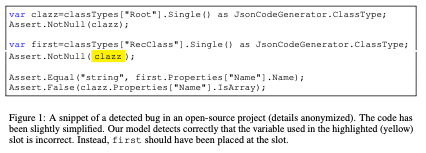
\includegraphics[width=\columnwidth]{Images/Background1.png}}
\label{icml-historical}
\end{center}
\vskip -0.2in
\end{figure}
In this section we will be focusing on representing programs as graphs. We are using the paper \cite{allamanis2017learning} to present the current state of the art procedure to represent programs as graphs for GNN processing. The authors present how to construct graphs from source code and how to scale Gated Graph Neural Networks training to such large graphs.We do this by encoding programs as graphs, in which edges represent syntactic relationships (e.g. “token before/after”) as well as semantic relationships (“variable last used/written here”, “formal parameter for argument is called stream”, etc.). They evaluate their method on two tasks: VARNAMING, in which a network attempts to predict the name of a variable given its usage, and VARMISUSE, in which the network learns to reason about selecting the correct variable that should be used at a given program location. The VARNAMING task, in which given some source code, the “correct” variable name is inferred as a sequence of subtokens. This requires some understanding of how a variable is used, i.e., requires reasoning about lines of code far apart in the source file. The variable misuse prediction task (VARMISUSE), aims to infer which variable should be used in a program location. To illustrate the task, Figure above shows a slightly simplified snippet of a bug their model detected in a popular open-source project. The Code used for experiments are published at https://github.com/dmitrykazhdan/Representing-Programs-with-Graphs.

\subsection{Formulation of task description}
In the proposed formulation a source code file is viewed as a sequence of tokens t$_0$ . . . t$_N$ = T , in which some tokens t$_{\lambda_0}$ , t$_{\lambda_1}$ . . . are variables. Furthermore, let V$_t$ $\subset$ V refer to the set of all type-correct variables in scope at the location of t, i.e., those variables that can be used at t without raising a compiler error. They call the location t where they want to predict the correct variable usage a slot. A separate task is defined for each slot t$\lambda$: Given t$_0$ . . . t$_{\lambda-1}$ and t$_{\lambda+1}$, . . . , $\lambda_N$ , correctly select t$_\lambda$ from V$_{t_\lambda}$ . For training and evaluation purposes, a correct solution is one that simply matches the ground truth, but note that in practice, several possible assignments could be considered correct (i.e., when several variables refer to the same value in memory).

\subsection{Gates Graph Neural Networks}
A graph G = (V , E , X ) is composed of a set of nodes V, node features X, and a list of directed edge sets E = (E$_1$,...,E$_K$) where K is the number of edge types. Each v is annotated with a real-valued vector x(v) $\in$ R$^D$ representing the features of the node (e.g., the embedding of a string label of that node). Every node v is associated with a state vector h(v), initialized from the node label x(v). The sizes of the state vector and feature vector are typically the same To propagate information throughout the graph, “messages” of type k are sent from each v to its neighbors, where each message is computed from its current state vector as m$_k^{(v)}$ = f$_k$(h$^{(v)}$). Here, f$_k$ can be an arbitrary function; A linear layer is chosen in this case. By computing messages for all graph edges at the same time, all states can be updated at the same time. In particular, a  new state for a node v is computed by aggregating all incoming messages as m$_k^{(v)}$ = g({m$_k^{(u)}$ | there is an edge of type k from u to v}). g is an aggregation function, on k as element wise summation. Given the aggregated message m$^{(v)}$) and the current state vector h(v) of node v, the state of the next time step h$'^{(v)}$ is computed as h$'^{(v)}$ = GRU(m$^{(v)}$, h$^{(v)}$), where GRU is the recurrent cell function of gated recurrent unit (GRU). The dynamics defined by the above equations are repeated for a fixed number of time steps. Finally, the state vectors from the last time step are the node representation.

\subsection{Program Graphs}
The backbone of a program graph is the program’s abstract syntax tree (AST). Add NextToken edges connecting each syntax token to its successor. Let a token v, let D$^R$(v) be the set of syntax tokens at which the variable could have been used last. Similarly, let D$^W$ (v) be the set of syntax tokens at which the variable was last written to. Graph to chain all uses of the same variable using LastLexicalUse edges. Return tokens are connected to the method declaration using ReturnsTo edges. While, arguments in method calls are connected to the formal parameters that they are matched to with FormalArgName edges. The authors introduce their respective backwards edges (transposing the adjacency matrix), doubling the number of edges and edge types

\subsection{Leveraging Variable Type Information}
The authors assume that a statically typed language and that the source code can be compiled, and thus each variable has a (known) type $\tau$(v). To use it, a learnable embedding function r($\tau$) for known types and additionally define an “UNKTYPE” for all unknown/unrepresented types. Rich type hierarchy that is available in many object-oriented languages is also taken into account. They map a variable’s type $\tau$(v) to the set of its supertypes, i.e. $\tau^\ast$(v) = {$\tau$: $\tau$(v) implements type $\tau$} $\cup$ {$\tau$(v)}. Then the type representation r$^\ast$(v) of a variable v as the element-wise maximum of {r($\tau$) : $\tau$ $\in$ $\tau^\ast$(v)} is computed. the maximum is chosen as it is a natural pooling operation for representing partial ordering relations (such as type lattices). Using all types in $\tau^\ast$(v) allows us to generalize to unseen types that implement common supertypes or interface. These types implement a common interface (IList) and share common characteristics.

\subsection{Initial Node Representation}
The poposed method splits the name of a node into subtokens (e.g. classTypes will be split into two subtokens class and types) on camelCase and pascal case. Then average is taken of the embeddings of all subtokens to retrieve an embedding for the node name. Finally, the learned type representation r$^{\ast}$(v) is concatenated.

\subsection{Programs Graphs for VarNaming}
Given a program and an existing variable v, They build a program graph as discussed above and then replace the variable name in all corresponding variable tokens by a special <SLOT> token. The initial node labels computed is used as the concatenation of learnable token embeddings and type embeddings as discussed above, GGNN propagation is repeated for 8 time steps and then variable usage representation by averaging the representations for all <SLOT> tokens is computed. This representation is then used as the initial state of a one-layer GRU, which predicts the target name as a sequence of subtoken.

\subsection{Programs Graphs for VarMisuse}
To model VARMISUSE with program graphs, the graph is modified. First, to compute a context representation c(t) for a slot t where the used variable is predicted, a new node v$_{<SLOT>}$ at the position of t is inserted, corresponding to a “hole” at this point, and connection is made to the remaining graph using all applicable edges that do not depend on the chosen variable at the slot (i.e., everything but LastUse, LastWrite, and LastLexicalUse edges). Then, to compute the usage representation u(t, v) of of each candidate variable v at the target slot, a “candidate” node v$_{t,v}$ for all v in V$_t$ is inserted, and connected to the graph by inserting the LastUse, LastWrite and LastLexicalUse edges that would be used if the variable were to be used at this slot. Each of these candidate nodes represents the speculative placement of the variable within the scope.
Using the initial node representations, concatenated with an extra bit that is set to one for the candidate nodes v$_{t,v}$ , The GGNN propagation is repeated for 8 time steps. The context and usage representation are then the final node states of the nodes, i.e., c(t) = h($^{v_{<SLOT>}}$) and u(t,v) = h$^{(v_t,v)}$. Finally, the correct variable usage at the location is computed as arg maxv c(t)$^T$ u(t, v). The model is trained using maximum likelihood.

\section{Decompilation}
\label{decompilation}

\subsection{Introduction}
Compiled languages are languages whose source code is compiled into machine understandable code by compilers. This machine code can directly be read and executed by the processor. This low-level machine code can either be in binary form or some other intermediate form. Due to the compilation process, these languages are generally faster and more efficient in addition to giving fine-grained control over hardware variables like memory, CPU and GPU, etc. Most popular compiled languages include Java, C, C++, Go, Rust, etc. The process of converting high level source code into low level machine code or other intermediate formats is called Compilation. This is achieved by compilers and is pretty straight forward once we have access to the language specific compiler.

Naturally, the inverse process involves taking machine code in binary format and retrieving the source code. This inverse process is called Decompilation. This process is not so trivial and involves many complex challenges. The semantics of the high level programming language are often lost during compilation. \citet{coda} state that there are both intra-statement and inter-statement dependencies in the low-level instructions that need to be preserved by the decompiler. Although challenging, Decompilation is necessary in a variety of applications. Security analysis is crucial for low level code, and decompilation can help in areas like malware analysis and vulnerable software patching as presented in \citet{kolbitsch2009effective} and \citet{yakdan2016helping}. Moreover, \citet{lee2011tie} show that malicious attackers can use decompilers to reverse engineer low level code and exploit commercial software. \citet{katz2019towards} also mention that decompilation can be useful for porting code to different hardware as well as source level analysis and optimization tools. Hence, having efficient and accurate decompilation tools can be of utmost importance.

\subsection{Conventional Decompilers}
Lots of research have been done for Decompilers over the years \cite{cifuentes1994reverse, emmerik2004using,brumley2011bap,bao2014byteweight,rosenblum2008learning,yakdan2016helping,brumley2013native}. Many rule-based and pattern matching decompilers have been developed like Hex-Rays \cite{hexray}, Phoenix \cite{brumley2013native} and the most recent one RetDec \cite{kvroustek2017retdec}. These compilers use pre-defined rules to match patterns in the low level code to control flow graphs of the high level code and translate the instructions accordingly. When such patterns are not found, the decompiler uses \textit{goto} statements in C. This is just like a line-to-line translation from low level code to C. Some decompilers like DREAM++ \cite{yakdan2015no,yakdan2016helping} exist which do not use \textit{goto} statements. However, these are still hand crafted.

Such hand-crafted compilers face a variety of problems like:
\begin{itemize}
    \item Most of these decompilers are handcrafted for a specific source-target language pair. This requires a lot of effort in itself, and this effort has to be replicated for each new source-target pair for which we want to build a decompiler.
    \item The output high level code fails to preserve the functionality of the low level code in most cases.
    \item The output high level code is not semantically readable and often lacks human friendliness. It also fails to use abstractions to represent the high level code as humans do. As a result, the reversed code is often hard to interpret and use it in corresponding applications.
\end{itemize}

\subsection{Problem Definition}
\citet{coda} gives a nice technical definition of the problem which we can reuse here. Let $P$ denote the high level program and $\tau$ denote the compiler. Hence, we can get the low level code as $\phi = \tau(P)$. They define the decompiler $\tau^{-1}$ that satisfies $\tau(P^{'}) = \tau(P) \text{ where } P^{'} = \tau^{-1}(\phi)$.

\subsection{Data Generation}
Data generation for decompilation tasks is relatively trivial due to the free availability of compilers. However, there are still some challenges. Generating source-target pairs can be done by taking the source code and running it through a compiler to get the executable or low level code. Nuances involve selecting the source code, selecting the different architectures for the compiler, selecting whether to produce the executable or the assembly instructions, etc. 

\citet{katz2018using} suggest creating a database of source-target pairs by compiling programs using a customized compiler based on Clang and LLVM. This compiler pairs AST trees and subtrees of source code with the corresponding low level machine code output by the compiler.They constrain the pairs by adding the following restrictions - 112 or fewer binary low level tokens and 88 or fewer source code tokens. The programs they use for their dataset are from open source RPMs for Fedora containing C source code. Comprehensive details are provided in their paper.

\citet{katz2019towards} generate samples for their decompiler to train on using random code samples from a subset of the C programming language. They do this by sampling the grammar of the language. These samples are guaranteed to be syntactically and grammatically correct. They then compile their code samples using the provided compiler. Doing so results in a dataset of matching pairs of statement, one in C and the other in Lll , that can be used by the model for training and validation. Note the two differing approaches here - taking C code from open source repos vs. using sampling to generate C source code. 

\citet{coda} use a two-step approach to decompilation (which we will discuss later). To build the dataset for stage 1, they randomly generate 50,000 pairs of high level programs with their corresponding compiled low level code. The compilation occurs using clang with all optimizations disabled. The source code programs can be roughly classified into short and long programs with an average length of 15 and 30 each. Their corresponding tree representations have a maximum depth of 3. They also use real world programs like neural network construction programs in pytorch C++ API and Hacker’s Delight loop-free programs. The dataset for the next stage is constructed by injecting various types of errors into the high level program. 10-20\% token errors are injected. The locations for these errors are sampled randomly using a uniform distribution. Once again, detailed statistics and methods are provided in their paper.

N-Bref \cite{nbref} assess the performance of their model on various benchmarks by using both generated high level code using their dataset generator as well as code written by humans in the form of Leetcode solutions to Problems (2017). The binary low level code is assembled using the GNU binary utilities to obtain the assembly code. To generate ASTs for the high level C code, the authors implement a parser using clang compiler for python. Their dataset generator for generated samples is built on top of csmith \cite{yang2011finding} - a code generation tool for compiler debugging. Their dataset generator avoids expression collision (EC). For instance, unary operators like \textit{i++} are converted to binary operators like \textit{i = i + 1} and all while loops are converted to for loops. This improves performance and also reduces confusion. The dataset generator also has several hyperparameters to control the depth, size, nesting, etc of the high level code. Here also the code is compiled with no optimizations. Previous works \cite{brumley2013native,lee2011tie,lin2010automatic} also
disabled optimizations, because many optimizations change variable types and rewrite source code
(e.g. loop-invariant optimization) which will result in unfair accuracy evaluations. Their dataset is available to download from \url{https://www.dropbox.com/s/33fop57jjq0wwa9/POJ-104.tar.gz?dl=1}.

A common theme across approaches is to take high level source code (mostly in C) and use compilers with some flags to generate the corresponding dataset pairs. Each approach tunes some nuances to generate their own datasets, but at the high level they have a lot of similarities. For future research, it will be nice to have a common benchmark and dataset for decompilation tasks. A common benchmark will aid in unbiased comparison of different methods and will also help more people easily research novel methods once a common dataset is easily available.

\subsection{Evaluation}
There are many different ways to evaluate decompilation tasks. You could compare the difference between the original source code and the generated source code using something like Levenshtein edit distance (LD) \cite{hyyro2001explaining}. You could compare the output of the original source code and the generated source code by compiling and then executing the binaries. Other works use BLEU, edit distance ratio, and syntactic correctness ratio \cite{nguyen2013lexical}. We will take a look at some of the approaches used by papers that use neural methods for decompilation.

\citet{katz2018using} use a separate test dataset to evaluate their model. They feed their trained model sequences of binary input code. The model outputs a series of tokens corresponding to the predicted output in the source language C aka the generated C source code. They use two evaluation metrics to assess the quality of the C source code generated by their technique. Since they use RNNs, the first metric, perplexity, is based on the RNN’s internal sampled softmax loss function, as described in \citet{jean2014using}, and is used during RNN training. It is a measure of the accuracy of a probabilistic model in predicting a sample \cite{shannon2001mathematical}. They use the perplexity measurement as a proxy for RNN performance to determine when to end training. The second metric is
based on the Levenshtein edit distance between the sequence of tokens in the ground truth source code associated with a given binary sequence and the sequence of tokens output by the RNN. They use two variations on edit distance. First is to look at straight edit distance between the tokens in the prediction and those in the ground truth snippet. Second, to ensure differences in identifier names and constants do not influence results, they lex both the output translations and ground truth snippets to obtain sequences of token types and perform the edit distance calculation between corresponding sequences of token types. They report the average edit distance for the exact tokens predicted; the average edit distance for the types of tokens predicted; and the percent of predicted token sequences that match the ground truth token sequences perfectly, without post-processing.

On the other hand, \citet{katz2019towards} uses the deterministic nature of the compiler to evaluate their model. After translating the inputs, for each pair of input i and corresponding translation t (i.e. the decompiled code), they recompile t and compare the output to i. This allows them to keep track of progress and success rates, even when the correct translation is not known in advance. Exact details are described in the paper. Despite holding the ground-truth for the test set (the C used to generate the set), they decided not to compare the decompiled code to the ground-truth because in some cases, different C statements could be compiled to the same low-level code (e.g. the statements x = x + 1 and x++). They believe that their evaluation method allows for such occurrences and is closer to what would be applied in a real use-case.

\citet{coda} (Coda) assess the performance of their model on various synthetic benchmarks with different difficulty levels and real-world applications. Given the binary executable as the input, we use an open-source disassembler \cite{mips,redasm} for MIPS \cite{hennessy1982mips} and x86-64 \cite{guide2011intel} architecture to generate the corresponding assembly code that is fed to the model. They evaluate the performance of the Coda using two main metrics: token accuracy and program accuracy. Token accuracy is defined as the percentage of the predicted tokens in high-level Programming Language that match with the ground-truth ones. Program accuracy is defined as the ratio between the number of predicted programs with 100% token accuracy and the number of total recovered programs.

\cite{nbref} uses different metrics for different stages of their model. For the source code generation stage, they use token accuracy and the graph edit distance \cite{sanfeliu1983distance} without enforcing the match between predicted and ground truth AST on graph generation. The metric is fair to evaluate decompilation tasks as we remove all the Expression collision. For the data-type solver stage, they use two metrics: (i) macro accuracy and (ii) micro accuracy.

Often, these metrics are combined and calculated in ways that give the success rates of decompilation in percentages. The evaluation metrics and protocol seem to vary across different neural decompilation approaches. This makes consistent evaluation across different methods difficult. Since this is a fairly recent research area, a standard evaluation benchmark and metric along with the standard dataset proposed earlier will aid in moving research forward in this domain.

Next we will discuss the different neural decompilation approaches at a high level.

\subsection{RNN and Neural Machine Translation (NMT) based approaches}
RNNs have become very popular for sequential Machine Learning tasks like translation, question answering ,etc \cite{sutskever2014sequence}. RNNs have feedback loops which permit persistence of data which in turn allows sequential processing \cite{siegelmann1993foundations}. An unrolled recurrent neural network has a natural sequence-like structure which makes it well suited for translation tasks. There are several variations on RNNs including the LSTM \cite{hochreiter1997long} which has increasingly become the go-to RNN of choice. LSTMs help preserve long term dependencies and have shown major improvements when dealing with longer sequences. A particular variant of RNNs is the sequence to sequence model or the seq2seq, which takes in an input sequence and generates an output sequence. As you can imaging, such seq2seq models are very useful for tasks like natural language translation \cite{cho2014learning}.

Decompilation can be seen as a natural expansion of the language translation task, but for programming languages. Translation for programming languages can also include translating between two high level languages like Java and Python. But decompilation deals with translation between a high level language and a low level binary executable/machine code. 

\citet{katz2018using} is one of the first approaches to adapt seq2seq RNN models for decompilation. Their sequence-to-sequence model is composed of two recurrent neural networks: an encoder, which processes the input sequence, and a decoder,
which creates outputs. Further, the sequence-to-sequence model contains a hidden state, C, which summarizes the entire input sequence. The output is generated from the decoder by taking in the hidden state and the current input and yielding a probability distribution from an activation function like Softmax. To modify this model for decompilation, they make many changes in all steps of the pipeline including pre-processing, model architecture, post-processing, etc. The first step involves tokenization of the input-output pair i.e. the source-target pair of the high level code/ low level code pair. The appropriate tokenizer is chosen and built based on expert domain knowledge. The authors also use bucketing to separate out different lengths of the input sequence \cite{bucketing}. Each bucket has its own RNN comprising of the encoder and decoder. Exact details can be found in the paper. The pipeline for an input pair looks like this - 
\begin{itemize}
    \item The binary low level code is tokenized and converted to a list of integers corresponding to the indices in the dictionary for the low level code of the tokenizer.
    \item The list of integers goes through bucketing to choose the relevant bucket and RNN
    \item The list then goes through the encoder to generate a hidden state for the binary code.
    \item The decoder then takes this state and outputs a probability distribution representing tokens in the high level code. This distribution is then converted to a list of integers with the integers corresponding to the indices in the dictionary for the high level code in the tokenizer.
    \item The tokens for the high level code are retrieved and combined from that dictionary.
\end{itemize}

This approach does not take into consideration the differences between natural languages and programming languages, thus leading to ineffective results. For example, as \citet{katz2019towards} point out, the code they generate often cannot be compiled or is not equivalent to the original source code. This approach did however show the possibility of NMT for decompilation, and served as a stepping stone for the next approach proposed by \citet{katz2019towards}. 

\citet{katz2019towards} combines Neural Machine Translation (NMT) and Program analysis to improve the performance of their Neural Decompilation model and make it more practically useful and viable. They also propose a framework called TraFix that can automatically learn a decompiler from a compiler and check the correctness of the decompiler using a verifier. Their approach consists of two complimentary phases:
\begin{itemize}
    \item Generating a code template that, when compiled, matches the computation structure of
the input. The input is the low level binary code.
    \item Filling the template with values and constants that result in code equivalent to the input. This means that the output from running the executable will be the same for both cases.
\end{itemize}
They use a NMT model combined with a feedback loop which facilitates active learning based on the outputs of phase 1. Phase 1 results are compared to the computation structure of the input. If they match, the generated code moves to phase 2. If not, the dataset is updated and the model is trained again. The authors use LSTMs for their NMT model.

NMT based techniques are still primarily sequential and fail to incorporate the graph and tree structures of code like control flow graphs and abstract syntax trees. We will take a look at some newer methods which try to incorporate these properties.

\subsection{Abstract Syntax Tree (AST) based Neural Decompilation}
Coda \cite{coda} also uses a two phase learning approach and an NMT model at its base. But it tries to incorporate the code structure into the encoder and decoder of the RNN. Its two phase approach can be described as:
\begin{itemize}
    \item It uses an instruction type-aware encoder and a abstract syntax tree (AST) decoder
for translating the input binary into the target PL. Their encoder deploys separate RNNs for different
types of statements, thus the statement boundaries are preserved (This is different from bucketing used by \citet{katz2019towards}. Furthermore, the control and data dependency in the input program are translated to the connections between the hidden states of corresponding RNNs. The output from the AST decoder maintains the dependency constraints and statement boundaries using terminal nodes, which facilitates learning the grammar of the target PL.
    
    \item In this stage, Coda employs an RNN-based error predictor (EP) to identify potential
prediction mistakes in the output program from Phase 1. Ensembling method can be used to boost
the performance of the error prediction. The EP is used to guide the iterative correction of the output
program. Unlike traditional decompilers which utilize only the syntax information from the input,
Coda leverages the Levenshtein edit distance (LD) between the compilation of the updated output
program and the ground-truth low-level code to prevent false alarms induced by the EP. This can be considered conceptually similar to phase 2 of \citet{katz2019towards}.

They also employ a technique called Attention Feeding to combine different contexts in the AST decoder. This can be considered similar to message passing in graphs, since trees are a form of graph. The Attention Feeding is comprised of parent attention feeding and input instruction attention feeding. Parent feeding refers to context from the parent of the current node, and input feeding refers to context from the current node's corresponding node in the input.
\end{itemize}

\subsection{Bringing Graph Neural Networks into the picture}
Even after incorporating AST structure, the base models of the previous approach are still derived from natural language based seq2seq models. This disregards the intrinsic structure of code (graphs/trees). To the best of our knowledge, \cite{nbref} is the first Neural Decompilation approach which utilizes Graph Neural Networks (GNNs) to represent code in the context of decompilation. They use a backbone structural transformer \cite{vaswani2017attention} with inductive Graph Neural Networks \cite{hamilton2017inductive} to represent the low-level code (LLC) as control/dataflow dependency graphs and source code as Abstract Syntax Tree (AST).

Their pipeline also involves a two step approach - data type solver (DT-Solver) and source code generator (SC-Gen). The output of the data type solver is used as the decoder input of the source
code generation. Both use the same backbone with GNNs.

\textbf{Structural Transformer with GNNs}
The backbone structural transformer has three components: (1) LLC encoder, (2) AST encoder, and (3) AST decoder. The LLC encoder takes the low-level instructions converted from binaries using disassembler as input. AST encoder takes the input of a previous (partial) AST, and the predictions of AST decoder are AST nodes, which can be equivalently converted to the high-level program. Here we will focus on the encoders and how they use GNNs. The GNN of choice in this paper is GraphSAGE (\citet{hamilton2017inductive}). GNNs are used in two places - 1) To embed the initial code/AST structure 2) To augment the Attention Layers in the Transformer



\textbf{Initial GNN embeddings}
The LLC encoder converts the initial low level code into a graph where each node is representated by its feature vector including features like register / instruction type ($var_t$
/ $ins_t$), position in the instruction ($n_{pos}$), node id ($n_{id}$) and numerical field ($n_{num}$). Edges are generated using hand crafted rules. Aggregation is done using max pooling. Aggregation vector and current state of the node are fed into a fully connected layer to get the next state. 3 layers are used for the GNN.

The AST encoder encodes the AST tree from the AST decoder to guide future
tree expansions. They treat the AST tree as a graph (V) and embed it using GraphSAGE as well. The input of the GNN includes meta-features of the tokenized AST node and a boolean indicating whether the node is expanded in this step. The output hidden states from the GNN is fed into the self-attention module. At the end of the AST encoder, they integrate the AST encoder output and LLC encoder output using an additional multi-head attention layer.


\textbf{GNN Augmentation for Attention}
The output of the attention layers is converted to a graph using the same edge rules in the LLC encoder and those states are then fed again into the GNN to obtain embeddings that incorporate the inductive biases of GNNs.

Experiments show that Nbref outperforms the corresponding transformer baseline and previous Neural Decompilers like Coda \cite{coda}. It also outperforms other models on human written Leetcode solutions. The performance gain over baseline Transformer clearly shows the value of using GNNs. Since most state of the art NMT models use transformers now, performance gains over previous Neural Decompilers using RNNs is expected. 

Critics for Nbref have mentioned that they do not propose anything novel, but the use of GNN based representations in Neural Decompilation is definitely the first we have come across. GNNs to represent code is a natural choice in many domains related to programming languages because of the graph and tree based structure of code. We believe future research will definitely involve the use of GNNs for learning representations of code. The way this is done might be tailored differently for decompilation to improve performance and efficiency. Once again, a common dataset and benchmark may help accelerate research in Neural Decompilation. 

\section{CodeXGlue}
Benchmarks in Natural Language Processing have played an important role in the progress of the field. Particularly, GLUE \cite{wang2018glue} is a comprehensive benchmark for training, evaluating and analyzing natural language understanding systems. It includes 9 tasks with corresponding datasets and evaluation guidelines, a diagnostic dataset to analyze NLP systems and a public leaderboard to track progress in the field. As expected, Deep Learning systems have dominated the benchmark and even surpassed human performance. As a result of this, SuperGLUE \cite{wang2019superglue} has been released as a continuation of GLUE with harder challenges in order to further progress the field.

Benchmarks provide a unified and system agnostic way for several different researchers to compare their approaches on a common ground. Most NLP papers dealing with finetuning language models will mention GLUE or SuperGLUE, and publish their results to the public leaderboard \footnote{https://gluebenchmark.com/leaderboard}. Looking at the incredible success of such benchmarks in NLP warrants a similar benchmark in applying Machine Learning to the domain of Programming Languages and Code. That is precisely what the recently released CodeXGlue (\citet{lu2021codexglue}) aims to achieve. Similar to GLUE, CodeXGlue contains a bunch of tasks paired with their corresponding processed datasets and a public leaderboard. The leaderboard can be found at \url{https://microsoft.github.io/CodeXGLUE/} and the github repo is at \url{https://github.com/microsoft/CodeXGLUE}.

We have so far discussed many domains of Programming Languages across which Deep Learning and Graph Neural Networks have shown tremendous potential. Now, we intend to cover this benchmark as a unifying evaluation point that will guide further research in applying Deep Learning and GNNs to the domain of programming languages. We will cover the tasks of the benchmark in brevity and also include short descriptions of the baselines. We will end this section by looking at how Graph Neural Networks can be utilized to vastly improve scores across all tasks in the benchmark. We hope this will serve as viable research direction for interested people.

\subsection{Tasks}
CodeXGlue includes 14 datasets for 10 diversified code intelligence tasks covering the following scenarios:
\begin{itemize}
    \item code-code (clone detection, defect detection, cloze test, code completion, code repair, and code-to-code translation)
    \item text-code (natural language code search, text-to-code generation)
    \item code-text (code summarization)
    \item text-text (documentation translation)
\end{itemize}

The tasks can be summarized in Fig. ....... which is taken from their github repo. The last category of tasks \textit{text-text} leans more towards NLP but the rest contain code as their prime or major component. With code comes the intrinsic structure of programming languages including trees and graphs, and this varies greatly from natural languages. Therefore, we believe the inductive biases of Graph Neural Networks are very well suited to represent the code aspect in these tasks. Since this is a fairly recent benchmark, the leaderboard mostly contains baselines as of now. Most of the baselines mentioned in the CodeXGlue paper and papers like CodeBERT \cite{feng2020codebert} use transformer models which are directly adapted from their NLP counterparts. Hence, there is plenty of room for innovation and climbing the leaderboard on this benchmark. We will briefly cover the baselines and then see how Graph Neural Networks can be used to bolster these deep learning models.

\subsection{Baselines}
The baselines use different variants of Transformers as their backbone. The tasks can be approximately classified into understanding tasks like code search, code clone detection, defect detection, cloze test (similar to masked language modeling) and generative tasks like code repair, code translation, code completion, code generation, etc.

For code understanding tasks, the authors provide CodeBERT \cite{feng2020codebert} as a baseline. CodeBERT is very similar to BERT \cite{devlin2018bert} and treats programming language as sequential. The model is pretrained on the CodeSearchNet dataset \cite{husain2019codesearchnet} using a masked language modeling objective like BERT and a combination of comments and code as input. It is then fine tuned on the downstream CodeXGlue tasks.

For generative tasks like code generation and code completion, the authors provide CodeGPT as the baseline. CodeGPT is inspired from GPT2 \cite{radford2019better}. CodeGPT contains pre-trained monolingual models on Python and Java corpora from the CodeSearchNet dataset, which includes 1.1M Python functions and 1.6M Java methods. They provide two variants of this baseline, one trained from scratch and one using GPT2 as the starting point.

For tasks which are more seq2seq in nature like code translation, the authors provide a encoder-decoder baseline with CodeBERT as the encoder and a custom transformer as the decoder.

\subsection{Graph Neural Networks}
The baselines include models adapted from the NLP domain. As a result, the baselines treat code as natural language and disregards its intrinsic structure and syntactic biases. As we have seen throughout the paper, Graph Neural Networks have shown great promise in tasks related to programming languages. In section 1....... we saw the latest research in representing code using graph neural networks. In the rest of the sections, we saw how GNNs and representations using GNNs are adapted to specific domains. 

A lot of those techniques can be used across multiple tasks in CodeXGlue and we believe they can give consistent improvements as compared to the baselines. We will explore some ways that we envision GNNs being used across tasks in CodeXGlue.

\section{Program Similarity and Classification}
\label{similarity}
\subsection{Introduction}

Graph similarity search is one of the most important graph-based applications, with extensive applications to complex graph querying systems such as finding similar chemical compounds.
However, Graph Edit Distance (GED) and Maximum Common Subgraph (MCS), the core operations of graph similarity/distance computation are very costly in practice.
As graph databases become increasingly dense, it becomes paramount to be able to efficiently mine these large repositories for fundamental tasks of similarity computation and classification.
Additionally, domain specific relational graphs, expert knowledge and reasoning of both meaningful structure and semantics is required – suggesting the need for automation.

\subsection{SimGNN}
SimGNN \cite{bai2019simgnn} proposes
\begin{enumerate}
    \item Designing a learnable embedding function that maps every graph to an embedding vector.\\
        A Novel attention mechanism is utilized subject to a specific similarity metric
    \item Design a pairwise node comparison method to supplement the graph-level embeddings with find-grained node-level information
\end{enumerate}
Approach to speed-up graph-similarity computation by finding approximate values heuristically via a learnable mapping function. Resultant process is quadratic with respect to graph size, which is still among the most efficient methods for graph similarity computation.\\

Formally, the \textit{Graph Edit Distance} between $G_1, G_2 = GED(G_1, G_2)$, the number of edit operations in the optimal alignments that transform $G_1$ to $G_2$, where an edit operation is an insertion or deletion of a vertex/edge or relabelling of a vertex.
If two graphs are isomorphic, their GED is 0.\\
\subsubsection{Graph-Level Embedding}  Node embedding is generated via Graph Convolutional Network (GCN) specifically:\\ $conv(\mathbf{u_n}) = f_1(\sum_{m \in \mathcal{N}(n)}\frac{1}{\sqrt{d_nd_m}}\mathbf{u_mW_1^{(l)} + b_1^{(l)}})$
where $\mathcal{N}(n)$ is the set of one hop neighbors of a node $n$, $n$ inclusive, $d_n$ is the degree of node $n$ + 1 $\mathbf{W_1^{(l)}} \in \mathbb{R}^{D^l \times D^{l+1}}$ is the $l$-th layer weight matrix, $\mathbf{b_1^{(l)} \in \mathbb{R}^{D^{l+1}}}$ is the bias, and $f_1(\cdot)$ is an activation function.\\
Denote input node embeddings as $U \in \mathbb{R}^{N \times D}, u_n \in \mathbb{R}^D$ is the embedding of node $n$. Global graph context $c \in \mathbb{R}^D, c = tanh(\frac{1}{N}W_2\sum_{n=1}^Nu_n),\quad W_2 \in \mathbb{R}^{D \times D}$ is a learnable weight matrix. For a node $n$, to imbue awareness of global context $c$ in its attention $a_n$, take the inner product of the context $c$ and the node embedding
Graph Embedding $h \in \mathbb{R}^D$ is the attention weighted sum of the node embeddings: $h = \sum_{n=1}^N\sigma(u_n^Tc)u_n$.\\
\centerline{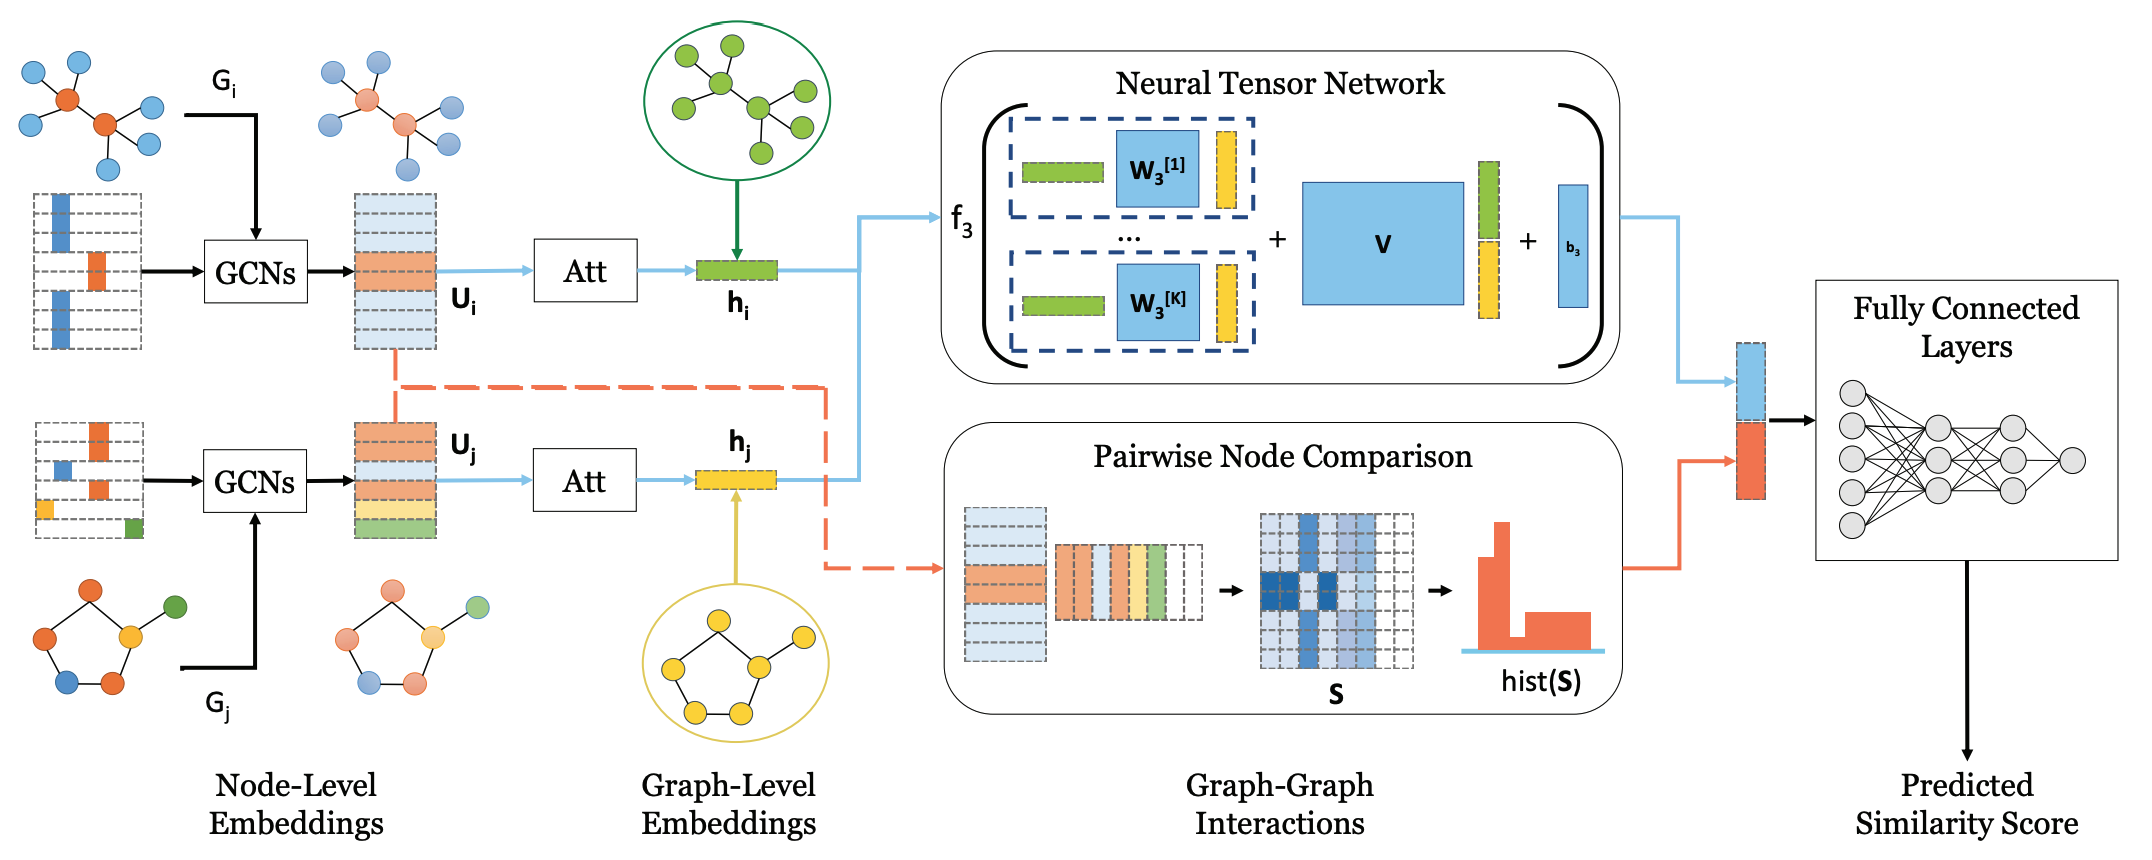
\includegraphics[width=\columnwidth]{Images/Similarity2-1.png}}
Use Neural Tensor Networks (NTN) to model the relation between two graph-level embeddings:
$g(h_i, h_j) = f_3(h_i^TW_3^{[1:k]}h_j + V\begin{bmatrix} h_1 \\ h_j \end{bmatrix} + b_3)$
where $W_3^{[1:k]} \in \mathbb{R}^{D \times D \times K}$ is a weight tensor, $[\cdot]$ is the concatenation operation.
$V \in \mathbb{R}^{K \times 2D}$ is a weight vector, $b_3 \in \mathbb{R}^K$ is a bias vector. $K$ is a hyperparameter controlling the number of interaction scores produced by the model for each graph embedding pair.\\
Feed these similarity scores into a Multi-Layer Perceptron (MLP) to one score $\hat{s}_{ij} \in \mathbb{R}$ to be compared directly in the loss function:
$\mathcal{L} = \frac{1}{|D|} \sum_{(i,j) \in D}(\hat{s}_{i,j} - s(G_i, G_j))^2$
where $D$ is the set of training graph pairs and $s(G_i, G_j)$ is the ground truth similarity.\\
\subsubsection{Pairwise Node Comparison}
To overcome limitations of graph-level embeddings (loss of node feature distribution and graph size) use the node embeddings directly.
Consider graphs $G_i, G_j$ with node embeddings $U_i \in \mathbb{R}^{N_i \times D}, U_j \in \mathbb{R}^{N_j \times D}$ with pairwise interaction scores $S = \sigma(U_iU_j^T)$, zero padding the smaller graph $\implies S \in \mathbb{R}^{N \times N}, N = max(N_i, N_j)$.
To ensure invariance to graph representations, histogram features $hist(S) \in \mathbb{R}^B$ are extracted, where $B$ is a hyperparameter indicating the number of bins. This histogram feature vector is normalized and concatenated with graph level interaction scores and fed to the fully connected layers.

\subsubsection{Evaluation}
Experiments conducted on the following datasets:
\begin{itemize}
    \item \textit{AIDS}: collection of antivirus screen chemical compounds containing 42,687 structures with Hydrogen omitted. Of these 700 were selected, having $\leq$ 10 nodes.
    \item \textit{LINUX}: 48,747 Program Dependence Graphs (PDG) generated from the Linux kernel. Each represents a function, where a node represents a statement and an edge represents the dependency of the statements. (10 nodes or less)
    \item \textit{IMDB}: 15000 ego-networks of actors/actresses, edges determined if they costared in the same film.
\end{itemize}
Shown here are the results for the \textit{LINUX} dataset across the \textit{Spearman's Rank Correlation Coefficient ($\rho$)}, \textit{Kendall's Rank Correlation Coefficient} ($\tau$), and \textit{precision at k} (p@k) – computed by taking the intersection of the top $k$ predicted and ground truth values divided by $k$.
It can be observed that SimGNN exhibits the best performance on \textit{LINUX} across all metrics.
\centerline{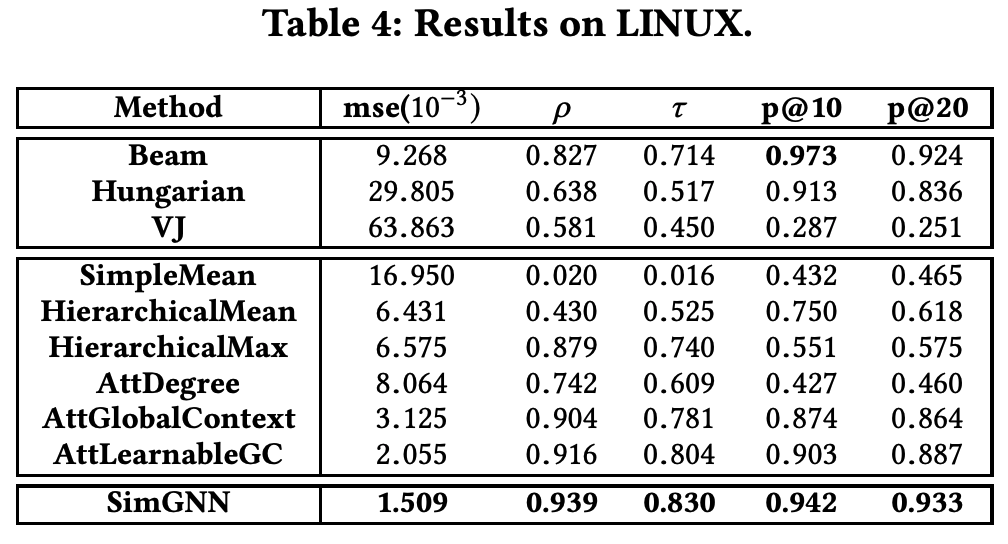
\includegraphics[width=\columnwidth]{Images/Similarity2-2.png}}
\subsubsection{Future Directions}
Work can be done to address the integration of edge features and scalability to larger graphs.

\subsection{Gated Graph Attention Neural Network (GGANN)}
Large scale online programming source code platforms such as Github are rapidly increasing both the number and size of their repositories – necessitating the ability to mine large codebases.
Proposed is the use of Abstract Syntax Trees (AST) to encode the syntactical structure of source code, even attaching data flow edges to encode semantic program meaning in the local scope.
To extend this concept to coarse-grained and global function-call relations, Gated Graph Attention Neural Networks \cite{lu2019program} are proposed. Contributions can be summarized as follows:
\begin{itemize}
    \item Program graph which integrates both data flow and function-call information into AST to characterize syntax and semantics
    \item Improvements made to GGNN model by introducing attention mechanism
\end{itemize}
\centerline{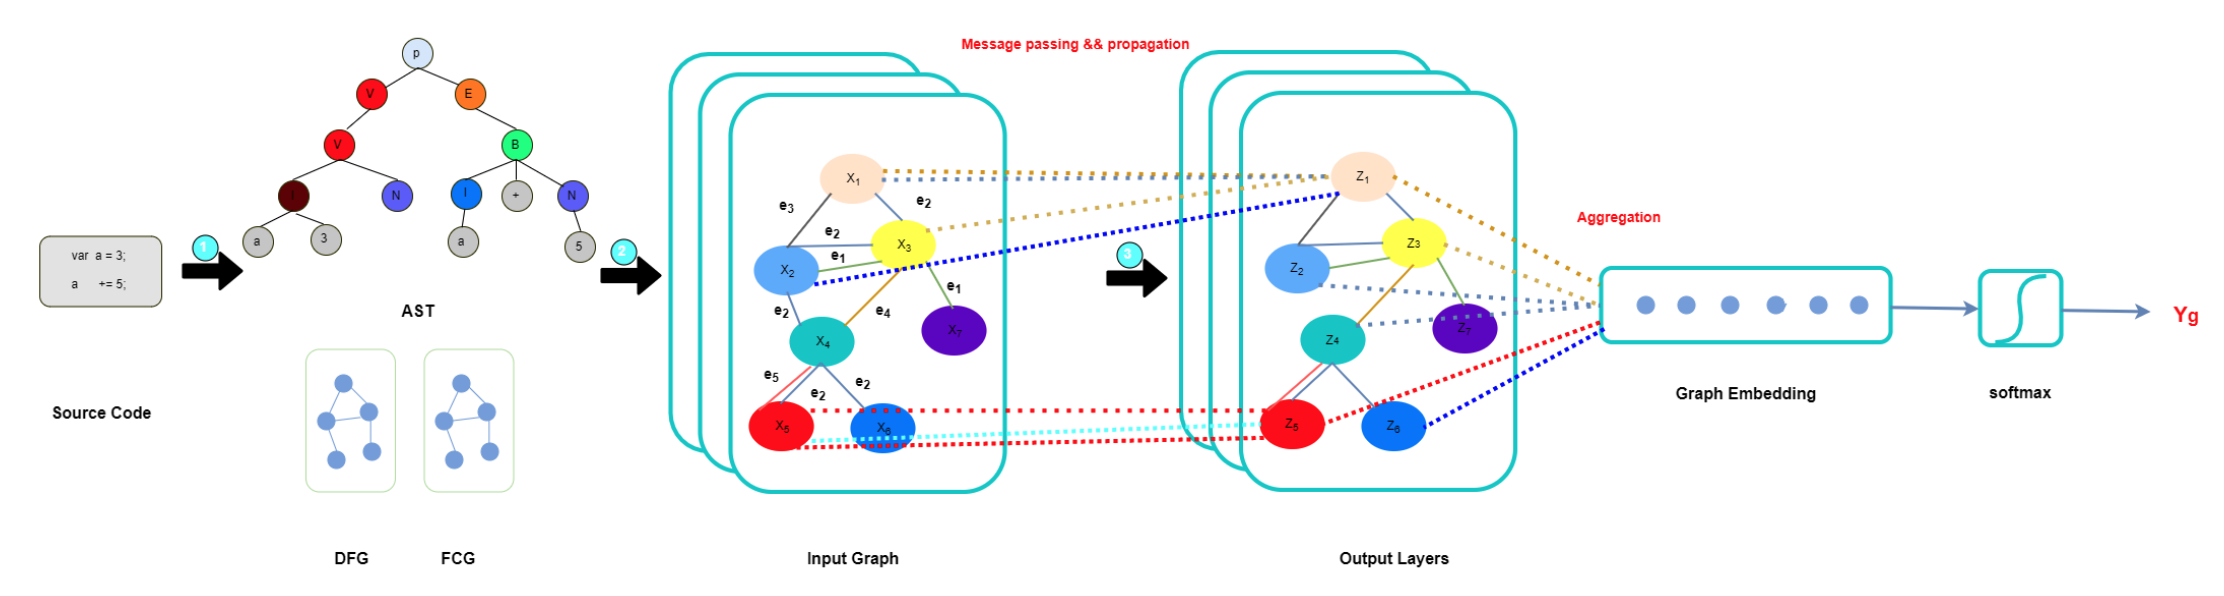
\includegraphics[width=\columnwidth]{Images/Similarity2-4.png}}
Directed graphs are represented as $G = (V,E)$ with edge type set $L_K = {l_1, l_2, \dots, l_k}$, connection matrix $A \in \mathbb{R}^{|V| \times 2|V|}$, where the element $A_{ij}$ is a $d \times d$ matrix, where $d$ represents the feature dimension of a node.
\centerline{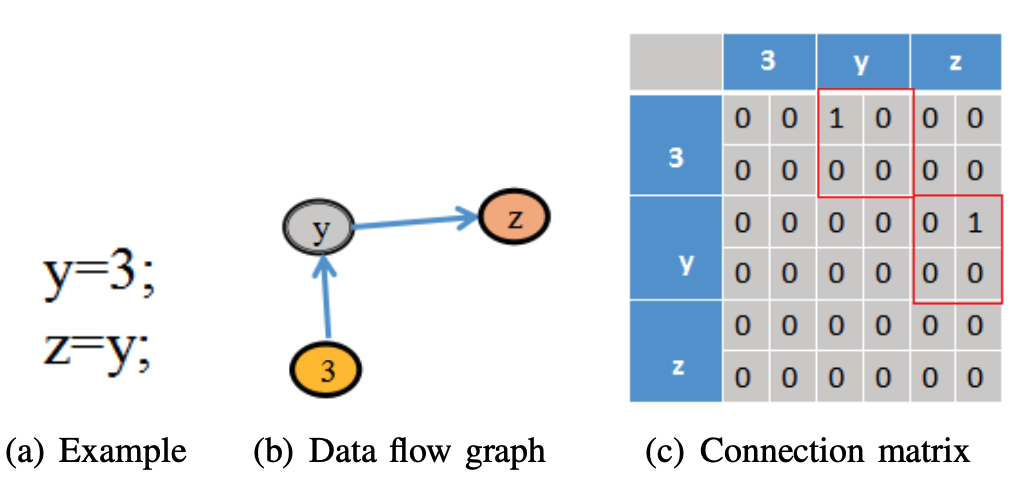
\includegraphics[width=\columnwidth]{Images/Similarity2-3.png}}
Directed graphs are represented as $G = (V,E)$ with edge type set $L_K = {l_1, l_2, \dots, l_k}$, connection matrix $A \in \mathbb{R}^{|V| \times 2|V|}$, where the element $A_{ij}$ is a $d \times d$ matrix, where $d$ represents the feature dimension of a node.
Neighbor state aggregation: $m_i^{(t)} = \sum\limits_{j \in N_i} A_{ij} \cdot h_j^{(t-1)}$ with per node state information: $h_i^{(t)} = GRU(m_t^{(t)}, h_i^{(t-1)})$
\subsubsection{Program Graph Construction}
Program graph construction consists of the construction of the AST, Function Call Graph (FCG), and Data Flow Graph (DFG).
AST is as described in preceding sections. Each node in FCG represents a function, while each edge denotes a function-call relation between two functions.
A node in DFG can be an entity, such as a variable, operator, structure identifier, etc., while an edge represents the data transfer between two entities.
\centerline{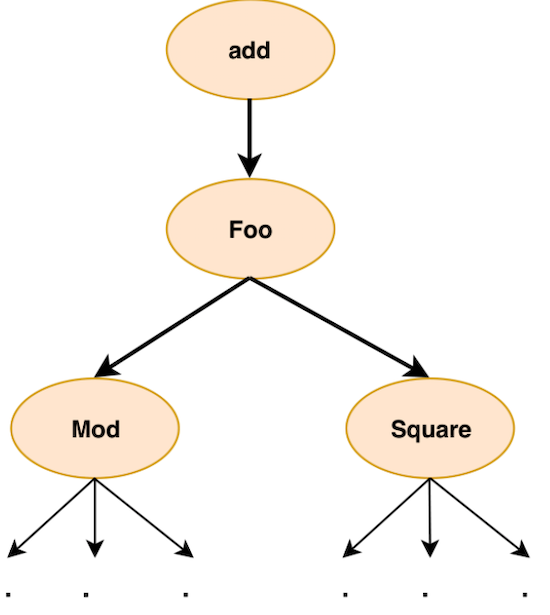
\includegraphics[width=\columnwidth]{Images/Similarity2-5a.png}}
\centerline{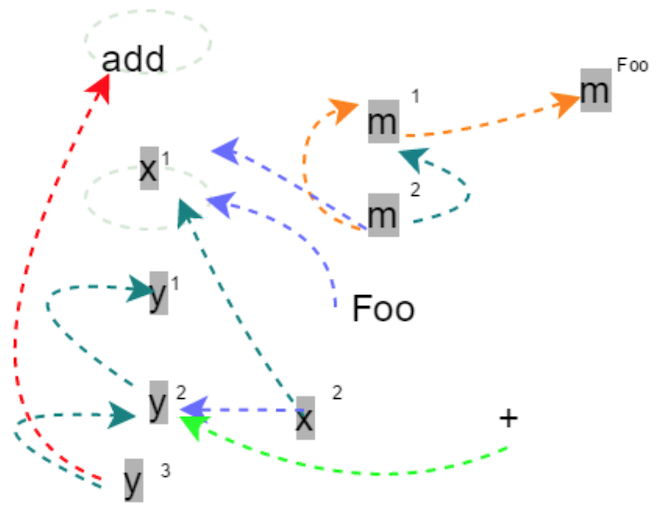
\includegraphics[width=\columnwidth]{Images/Similarity2-5b.png}}
It is desireable to integrate these representations into a new program graph that encapsulates their joint information: called the integrated FDA graph.
\centerline{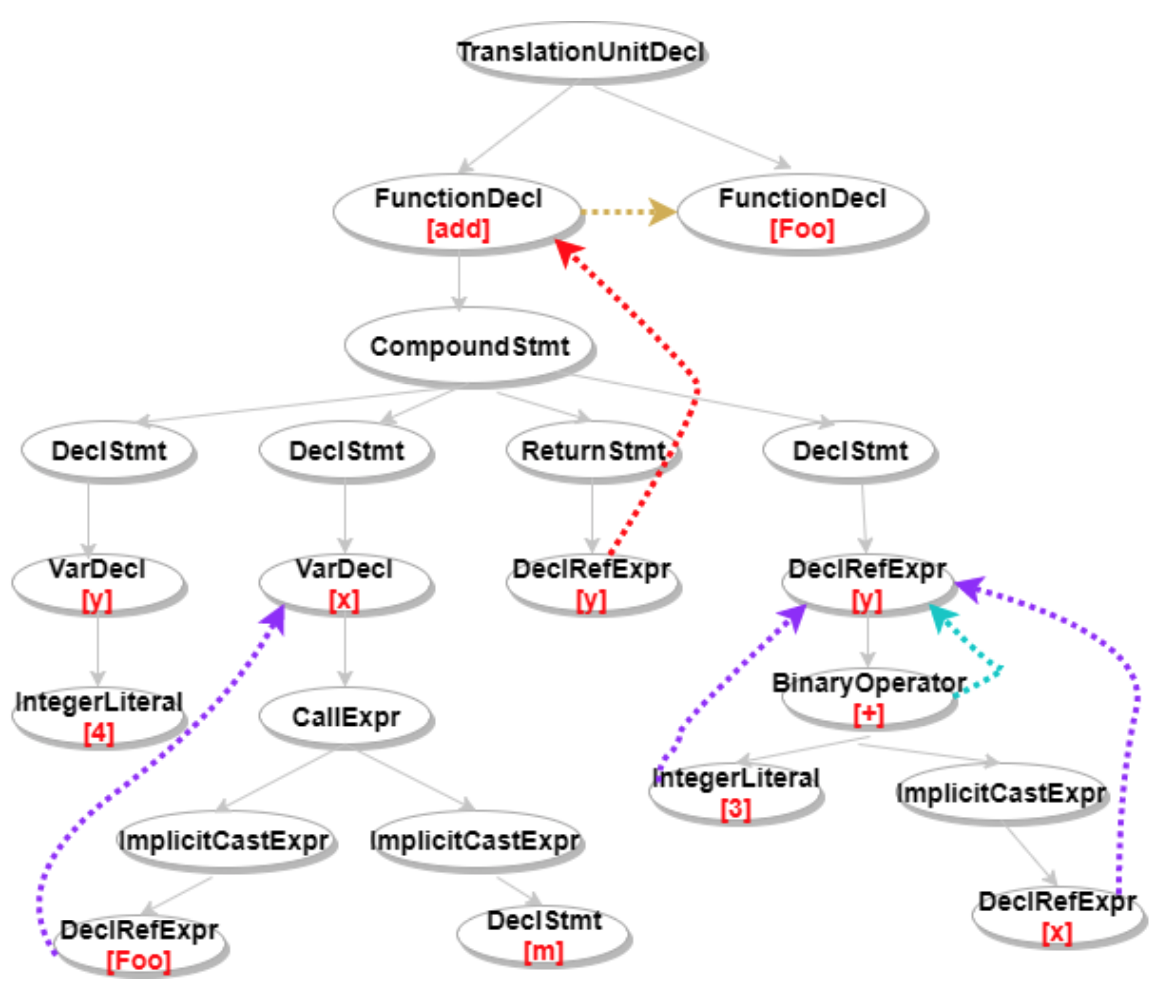
\includegraphics[width=\columnwidth]{Images/Similarity2-6.png}}
In summary, the node information aggregation is as follows:
$m_i^{(t)} = \sum\limits_{j \in N_i}\alpha_{ij} A(h_{ij}^{'(t)}) h_j^{(t-1)}$ with hidden state of directed edge $e_{ij}, \ h'_{ij} = U_e(h_{ij}^{'(t-1)}, h_i^{(t-1)}, h_j^{(t-1)})$ where $U_e$ is a multi-layer neural network.
Propagation matrix $A_{ij}$ can be replaced with a propagation matrix function, $A(h_{ij}') : \mathbb{R}^d \rightarrow \mathbb{R}^{d \times d}$ which learns the propagation matrix dynamically according to the dynamic information of the hidden state, realized by a multilayer neural network.
Information strength $\alpha_{ij} = softmax(a(h_i^{(t-1)}, h_j^{(t-1)}))$, where $a : \mathbb{R}^{d \times d} \rightarrow \mathbb{R}$ is an attention mechanism.
Vector representation for the FDA graph is unknown before calculation of the node's contribution, so it is approximated from the updated hidden state of each node after $T$ iterations of information propagation for sufficiently large $T$.
Embedding vector of the entire FDA graph can be evaluated by computing the weighted sum of node embeddings and an activation.
$h_G = softmax(\sum\limits_{i \in V}f(h_i^{(T)}, x_i) \odot g(h_i^{(T)}))$
\subsubsection{Experimental Evaluation}
Experiments were conducted on the Online Judge (OJ) programming source code files in C++, to be evaluated on classification accuracy, semantic analysis of learned representation, and attention analysis.
\centerline{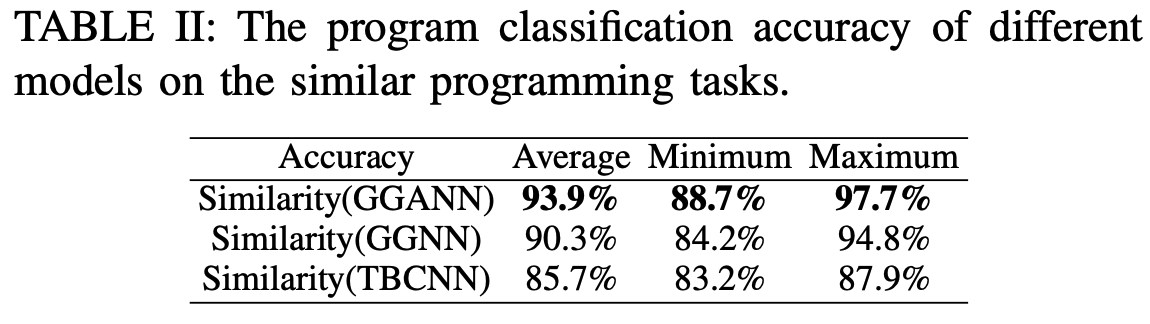
\includegraphics[width=\columnwidth]{Images/Similarity2-7.png}}
Node representations similarity was evaluated using K-means to see if similar nodes clustered into meaningful groups.
\centerline{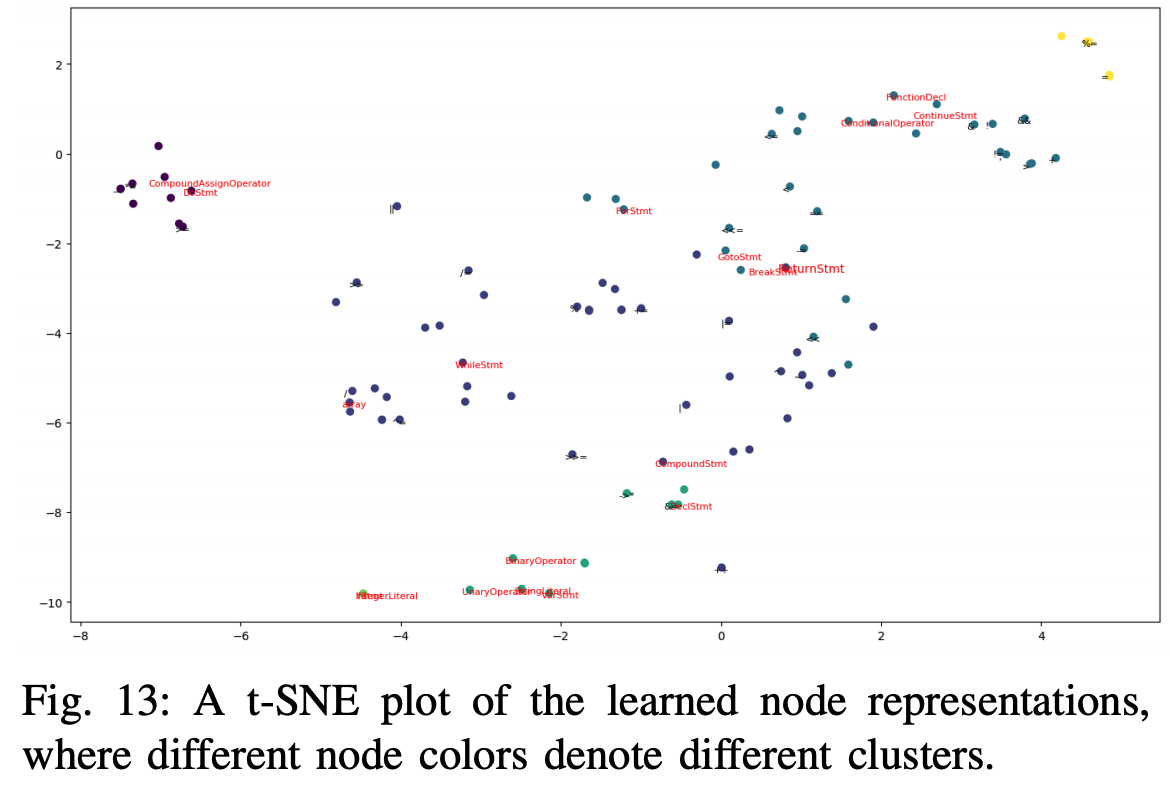
\includegraphics[width=\columnwidth]{Images/Similarity2-8.png}}
The attention mechanism was visualized via a heat map of the node attentions when aggregated to entire graph representations.
\centerline{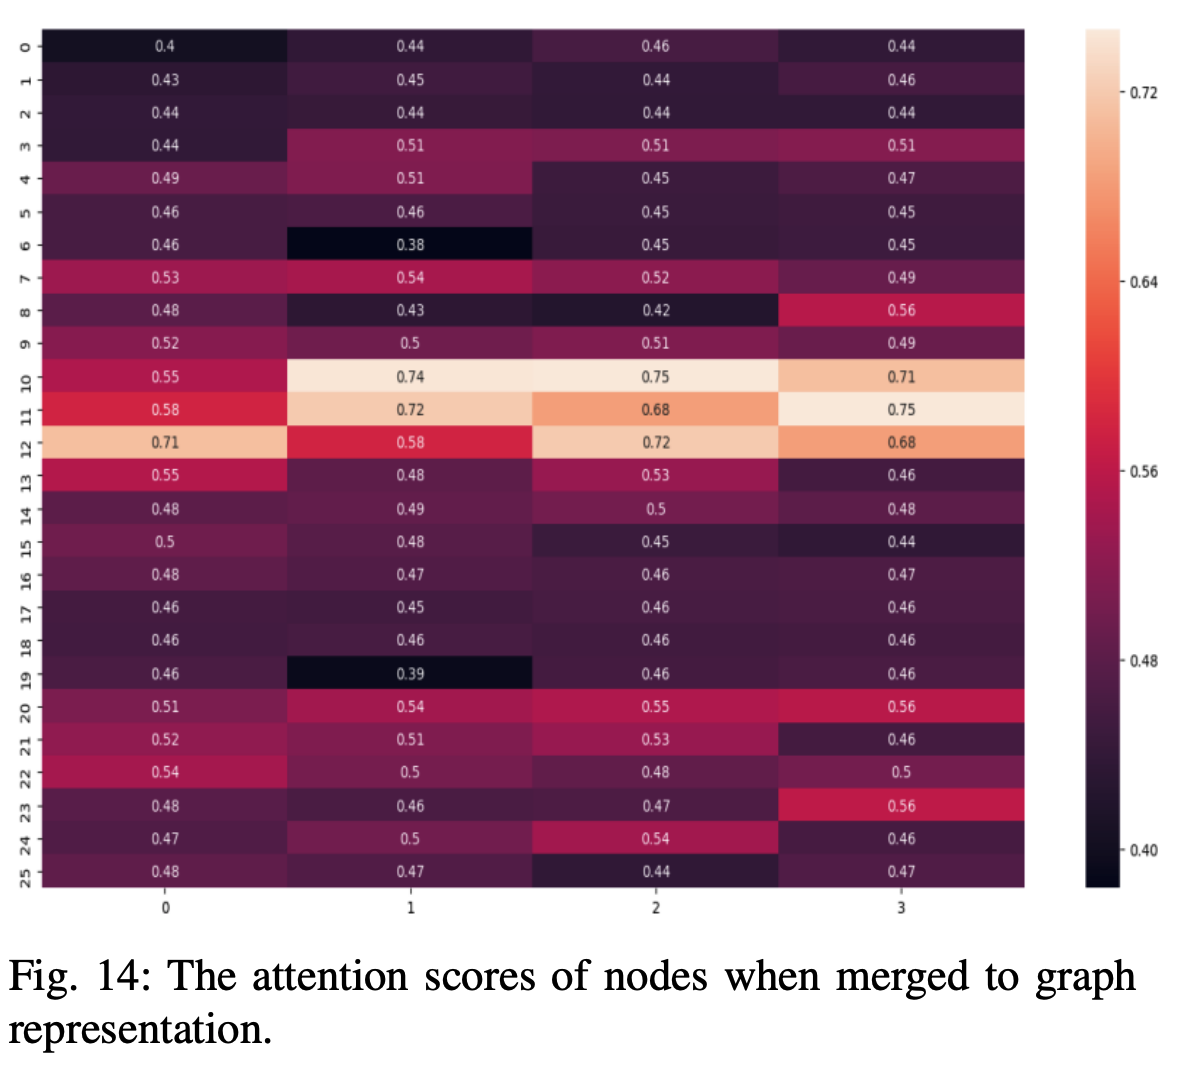
\includegraphics[width=\columnwidth]{Images/Similarity2-9.png}}

\subsection{Graph Matching Networks (GMN)}
Instead of computing graph representations independently for each graph, GMNs compute a similarity score through a cross-graph attention mechanism to associate nodes across graphs and identify differences.
Proposed models are evaluated on three tasks: a synthetic graph edit-distance learning task which captures structural similarity exclusively, and binary function similarity search and mesh retrieval, requiring added semantic similarity.
The contributions of the paper can be summarized as follows:
\begin{itemize}
    \item Demonstration of how GNNs can be used to produce graph embeddings for similarity learning
    \item Proposal of new Graph Matching Networks that compute similarity through cross-graph attention based matching
\end{itemize}
\subsubsection{Graph Embedding Models}
This GNN embedding model consists of an encoder, propagation layers, and an aggregator.\\
\textit{Encoder} maps the node and edge features to initial node and edge vectors through separate\\ MLPs:
$h_i^{(0)} = MLP_{node}(x_i) \  \forall i \in V \\
e_{ij} = MLP_{edge}(x_{ij}), \ \forall (i,j) \in E$\\
\textit{Propagation Layers}\\
$ m_{j \rightarrow i} = f_{message}(h_i^{(t)}, h_j^{(t)}, e_{ij})\\
h_i^{(t+1)} = f_{node}(h_i^{(t)}, \sum_{j:(j,i) \in E} m_{j \rightarrow i})
$ where $f_{message}$ is typically an MLP and $f_{node}$ can either be an MLP or a recurrent neural network core.\\
\textit{Aggregator}\\
After $T$ rounds of propagations, we compute the following graph level representation\\
$h_G = MLP_G(\sum\limits_{i \in V}\sigma(MLP_{gate}(h_i^{(T)}))\odot MLP(h_i^{(T)}))$ which transforms node representations and then uses a weighted sum with gating vectors to aggregate across nodes.
\subsubsection{Graph Matching Networks}
In this network, node updates will take into account aggregated messages at an inter/intra graph perspective, defined as follows
$ m_{j \rightarrow i} = f_{message}(h_i^{(t)}, h_j^{(t)}, e_{ij}), \forall (i,j) \in E_1 \cup E_2\\
  \mu_{j \rightarrow i} = f_{match}(h_i^{(t)}, h_j^{(t)}), \forall i \in V_1, j \in V_2, \text{ or } i \in V_2, j \in V_1\\
  h_i^{(t+1)} = f_{node}(h_i^{(t)}, \sum_j m_{j \rightarrow i}, \sum_{j'}\mu_{j' \rightarrow i})\\
  h_{G_1} = f_G({h_i^{(T)}}_{i \in V_1})\\
  h_{G_1} = f_G({h_i^{(T)}}_{i \in V_2})\\
  s = f_s(h_{G_1}, h_{G_2})\\
$
where $f_s$ is a standard vector space similarity and $f_{match}$ is a function that incorporates an attention based module:
$ a_{j \rightarrow i} = \frac{exp(s_h(h_i^{(t)}, h_j^{(t)}))}{\sum_j exp(s_h(h_i^{(t)}, h_j^{(t)}))}\\
  \mu_{j \rightarrow i} = a_{j \rightarrow i}(h_i^{(t)} - h_j^{(t)})
$ and therefore, \\
$\sum_j \mu_{j \rightarrow i} = \sum_j a_{j \rightarrow i}(h_i^{(t)} - h_j^{(t)}) =  h_i^{(t)} - a_{j \rightarrow i}h_j^{(t)}
$ with attention weights $a_{j \rightarrow i}$ and $\sum_j \mu_{j \rightarrow i}$ intuitively measures the difference between $h_i^{(t)}$ and its closest neighbor in the other graph.
The matching network has the ability to adjust its graph representations based on the compared graph, amplifying disparities if they do not match pairwise.
\subsubsection{Learning}
If similarity learning model is trained pairwise, samples must be labeled as similar and dissimilar, whereas triple training needs only relative similarity between the three samples.
Loss functions are defined respectively:
$L_{pair} = \mathbb{E}_{(G_1, G_2, t)}[max{0.\gamma-t(1-d(G_1,G_2))}]\\
 L_{triplet} = \mathbb{E}_{(G_1, G_2, G_3)}[ma{0,d(G_1,G_2)-d(G_1,G_3) + \gamma}]$
where $t$ is a binary similarity label.
\subsubsection{Evaluation}
Overall results demonstrate that GMns excel on graph similarity learning and consistently outperform other approaches, shown here is the binary function similarity search.
The model was evaluated on data generated by compiling an open source vido processing software \texttt{ffmpeg} using different compilers \texttt{gcc} and \texttt{clang} with various configurations.
\centerline{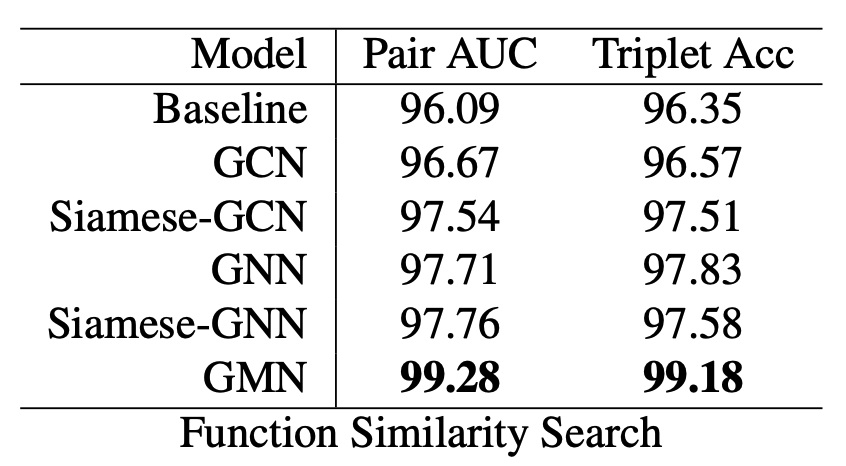
\includegraphics[width=\columnwidth]{Images/Similarity3-1.png}}

\subsection{Neural Code Comprehension \cite{ben2018neural}}
\subsubsection{Introduction}
A novel processing technique to learn code semantics, and apply it to a variety of program analysis tasks – based on an Intermediate Representation (IR), leveraging underlying data- and control-flow of programs.\\
\centerline{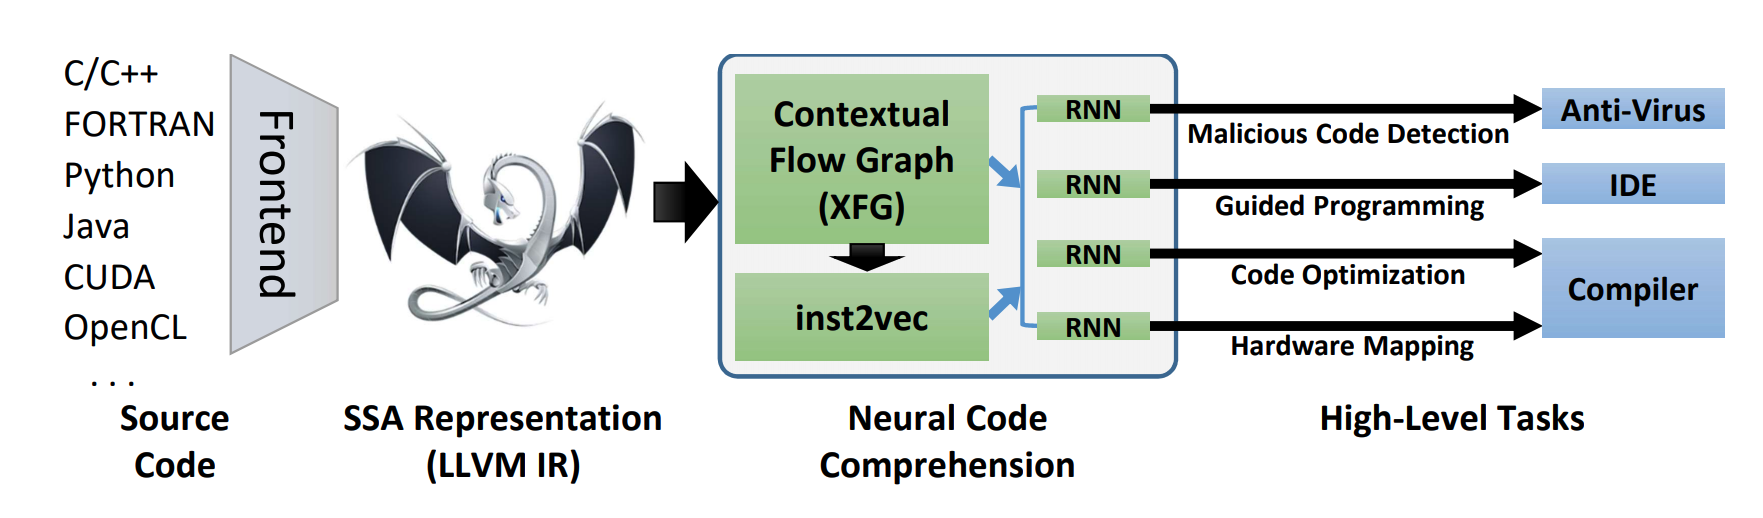
\includegraphics[width=\columnwidth]{Images/Similarity4-1.png}}
\textit{Naturalness Hypothesis: } Software is a form of human communication; software corpora have similar statistical properties to natural language corpora; and these properties can be exploited to build better software engineering tools
This work's contributions are as follows:
\begin{itemize}
    \item Formulation of a robust distributional hypothesis for code, from which a novel distributed representation of code statements based on contextual flow and LLVM IR is drawn.
    \item conteXtual Flow Graphs (XFGs): representation designed for statement embeddings that combine data and control flow
    \item Evaluation using clustering, analogies, semantic tests, and tasks
    \item Using simple LSTM architectures to show leading performance.
\end{itemize}
Robust Distributional Hypothesis of Code can be paraphrased as follows: Statements that occur in the same contexts tend to have similar semantics.
\subsubsection{Contextual Flow Processing}
XFGs are directed multigraphs that provide a notion of context, where nodes (variables or label identifiers) can be connected by more than one edge (data-dependence or execution dependence). 
\textit{XFG Construction}
\begin{enumerate}
    \item Read LLVM IR statements once, storing function names and return statements
    \item Second pass over the statements, adding nodes and edges according to the rule-set:
        \begin{enumerate}[(a)]
            \item Data dependencies within a basic block are connected
            \item Inter-block dependencies are both connected directly and through the label identifier 
            \item Identifiers without a dataflow parent are connected to their root (label or program root)
        \end{enumerate}
\end{enumerate}
\centerline{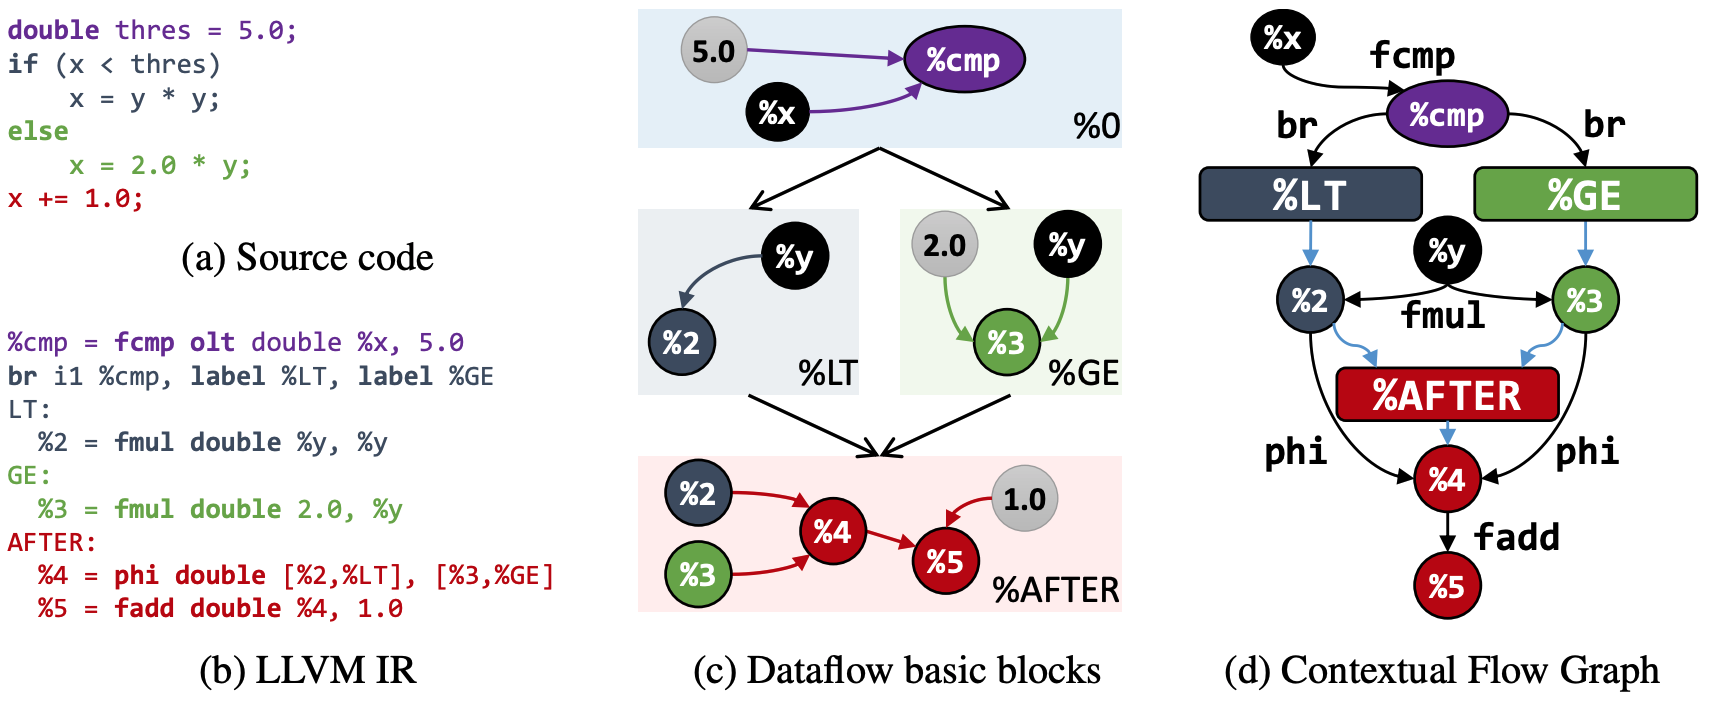
\includegraphics[width=\columnwidth]{Images/Similarity4-2.png}}
\subsubsection{inst2vec: Embedding Statements in Continuous Space}
Desiderata for an embedding space include: (a) statements that are in close proximity should have similar artifacts on a system (i.e. use the same resources); and (b) changing the same attributes (e.g. data type) for different instructions should result in a similar offset in the space.
\centerline{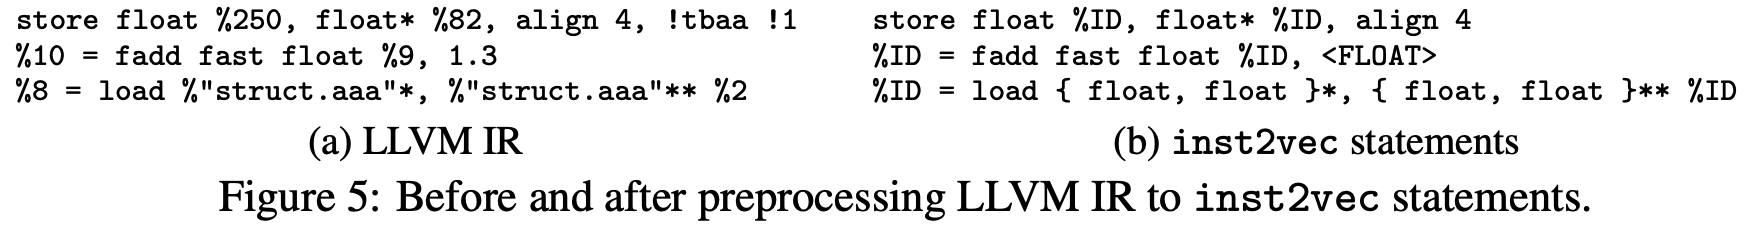
\includegraphics[width=\columnwidth]{Images/Similarity4-3.png}}
\texttt{inst2vec} was generated using corpora from different disciplines, even synthetically generated programs. Given a set of XFGs, neighboring statement pairs up to a certain context size via the skip-gram model are generated.
Pairs are obtained by constructing a dual graph in which statements are nodes, omitting duplicate edges.
\centerline{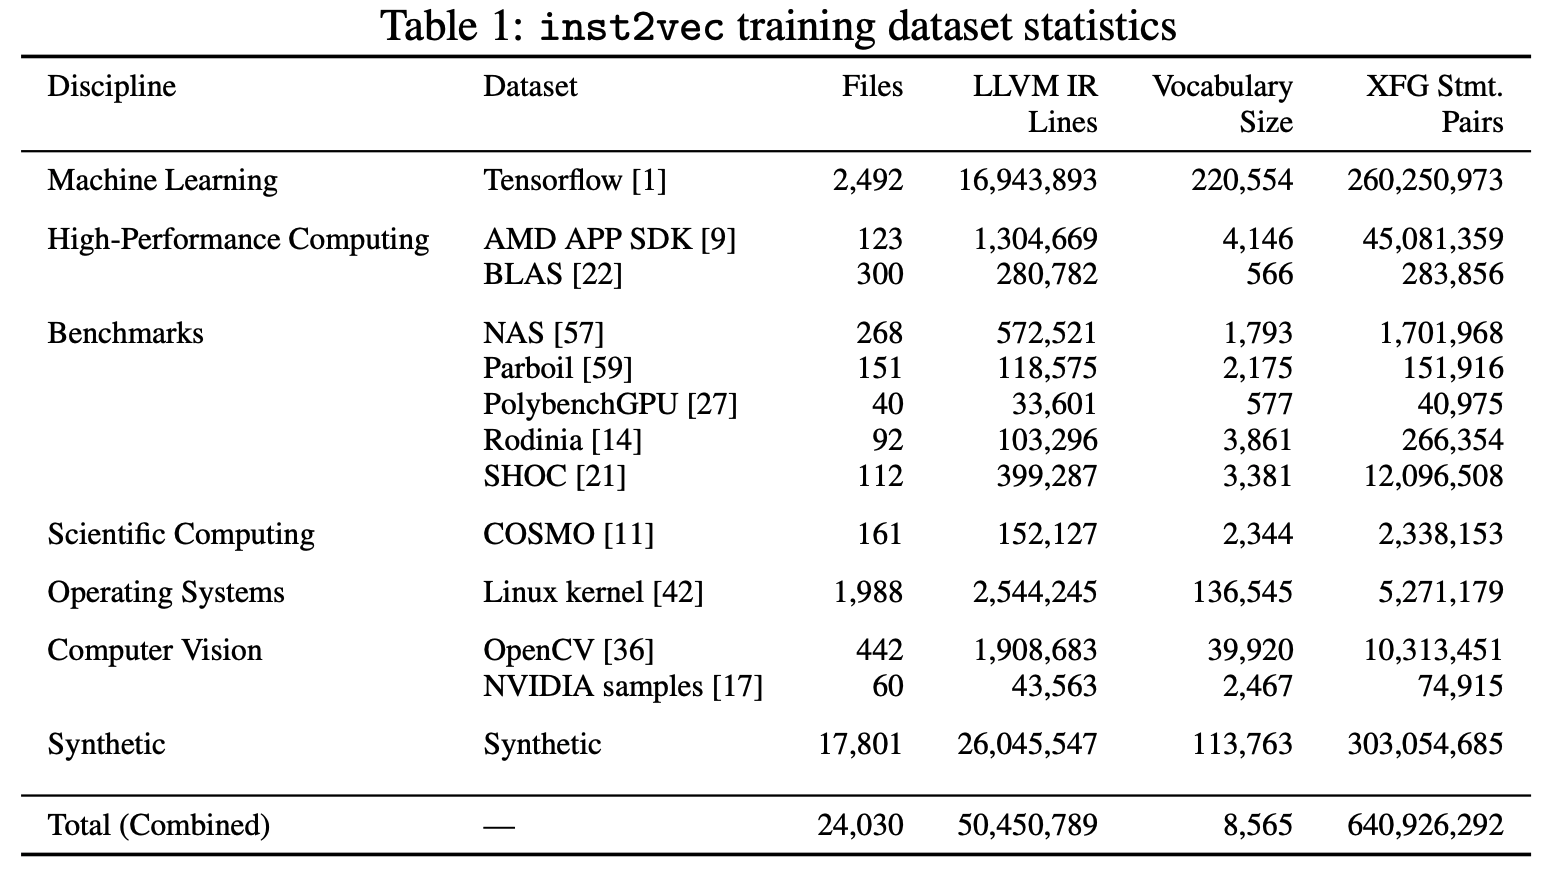
\includegraphics[width=\columnwidth]{Images/Similarity4-4.png}}
\subsubsection{Evaluation}
\centerline{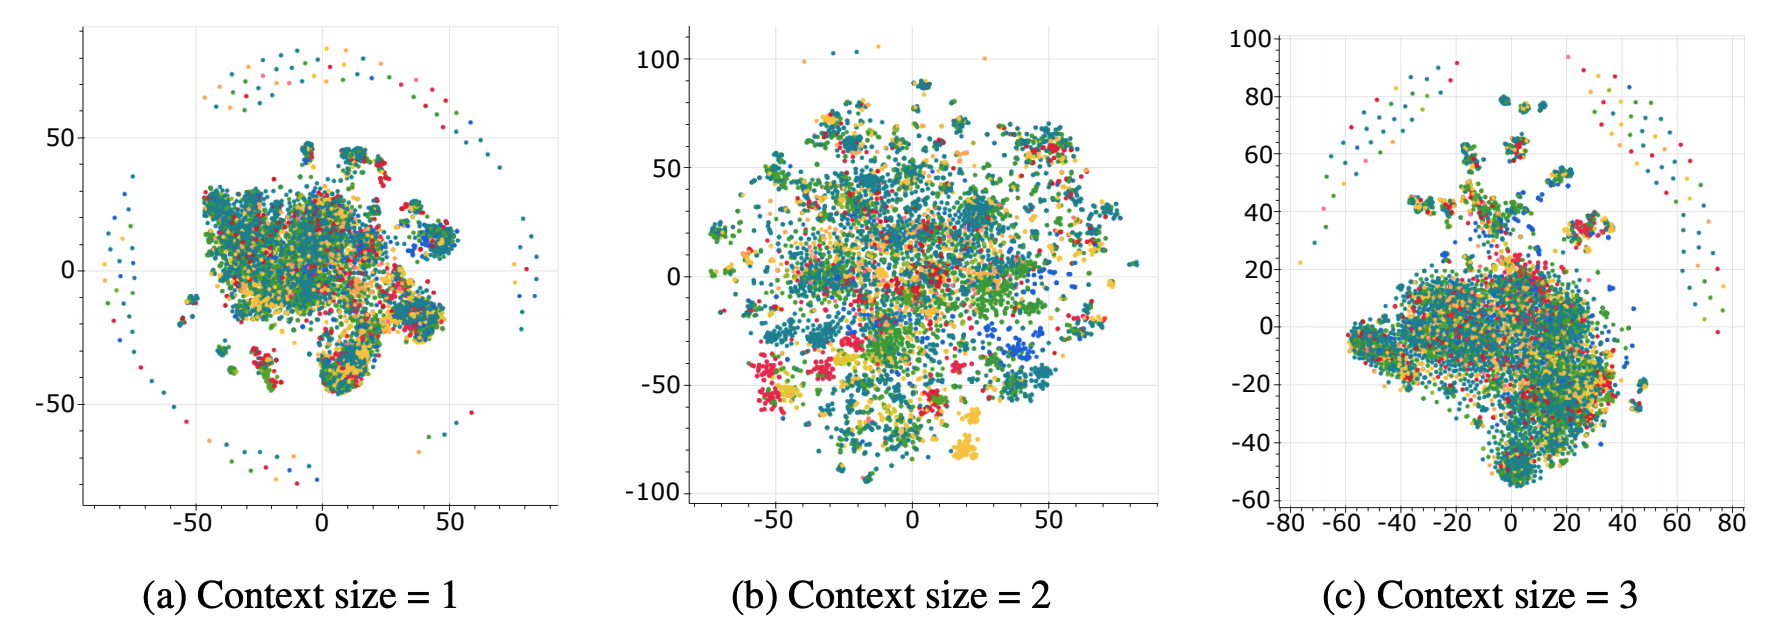
\includegraphics[width=\columnwidth]{Images/Similarity4-5.png}}
Using \texttt{inst2vec} an RNN was constructed that reads source code and outputs a predicted program class on the POJ-104 dataset, collected from the Pedagogical Open Judge System.
\centerline{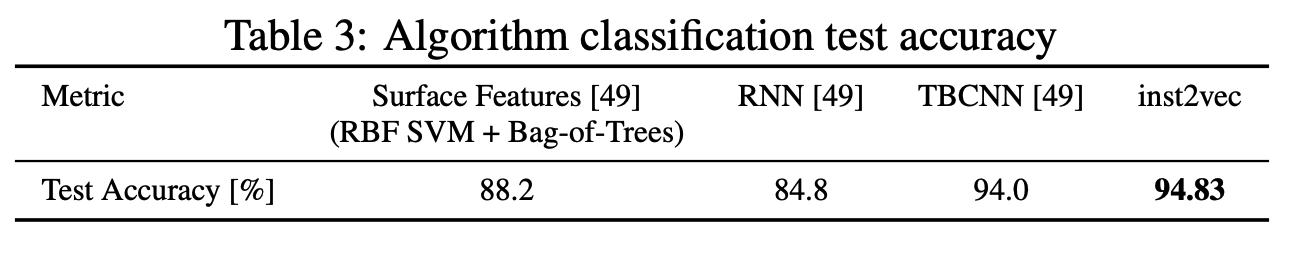
\includegraphics[width=\columnwidth]{Images/Similarity4-6.png}}

\section{Program synthesis}
\subsection{Introduction}
A general formulation of program synthesis called syntax-guided synthesis (SyGuS) seeks to synthesize a program that follows a given grammar and satisfies a given logical specification. Both the logical specification and the grammar have complex structures and can vary from task to task, posing significant challenges for learning across different tasks. Moreover, supervision is often unavailable for domain-specific synthesis tasks. To address these challenges, In this paper we suevey a metalearning framework that learns a transferable policy using only weak supervision. The program synthesizer takes as input a logical formula $\varphi$ and a grammar G, and produces as output a program in G that satisfies $\varphi$. In this formulation, $\varphi$ constitutes a semantic specification that describes the desired functional requirements, and G is a syntactic specification that constrains the space of possible programs.They assume a fixed grammar (i.e., syntactic specification G) across tasks.

Learning to understand and generate programs is an important building block for procedural artificial intelligence and more intelligent software engineering tools. It is also an interesting task in the research of structured prediction methods: while imbued with formal semantics and strict syntactic rules, natural source code carries aspects of natural languages, since it acts as a means of communicating intent among developers. Early works in the area have shown that approaches from natural language processing can be applied successfully to source code, whereas the programming languages community has had successes in focusing exclusively on formal semantics. More recently, methods handling both modalities (i.e., the formal and natural language aspects) have shown successes on important software engineering tasks and semantic parsing. However, current generative models of source code mostly focus on only one of these modalities at a time. For example, program synthesis tools based on enumeration and deduction are successful at generating programs that satisfy some (usually incomplete) formal specification but are often obviously wrong on manual inspection, as they cannot distinguish unlikely from likely, “natural” programs. On the other hand, learned code models have succeeded in generating realistic-looking programs. However, these programs often fail to be semantically relevant, because variables are not used consistently.

Along with the aforementioned problems, many modern APIs have an incredibly steep learning curve, due to their hundreds of functions handling many arguments, obscure documentation, and frequently changing semantics. For APIs that perform data transformations, novices can often provide an I/O example demonstrating the desired transformation, but may be stuck on how to translate it to the API.
\subsection{Related work}
A large body of work has been dedicated to solving program synthesis problems. Numerous systems have been developed targeting a variety of domains such as string processing [\cite{Gulwani2011}; \cite{parisotto2017neuro-symbolic}], data wrangling [\cite{Feng2018}], data processing [\cite{Smith2016}], syntax transformations [\cite{Rolim2017}], database queries [\cite{Yaghmazadeh2017}] and bit-vector manipulations [\cite{Jha2010}]. One paper attempts to categorise these works at a coarse level according to the high-level synthesis strategy used in their respective systems. Then summarise how strategy of using neural-backed generators compares and relates to these strategies.

CEGIS [\cite{SolarLezama2008}] is a general framework for program synthesis that synthesizes programs satisfying a specification $\phi$. The basic algorithm involves two components: a synthesizer and verifier, where the synthesizer generates candidate programs and the verifier confirms whether the candidate is correct. The synthesizer also takes the space of possible candidates as an input, either explicitly or implicitly. This space may be defined in multiple ways, for example using syntactic definitions of valid programs [\cite{Alur2013}]. A large fraction of techniques, including ours, fall under this general CEGIS framework, with differing strategies for producing program candidates, which are broadly classified below.

Source code generation has been studied in a wide range of different settings [\cite{allamanis2018survey}]. Early works approach the task by generating code as sequences of tokens [\cite{hindle2016CACM}], whereas newer methods have focused on leveraging the known target grammar and generate code as trees [\cite{Maddison2014}]. While modern models succeed at generating “natural-looking” programs, they often fail to respect simple semantic rules. For example, variables are often used without initialization or written several times without being read inbetween.

\textbf{Neural program synthesis}
Several recent works have used neural networks to accelerate the discovery of desired programs. These include DeepCoder [\cite{balog2017deepcoder}], Bayou [\cite{murali2018neural}], RobustFill [\cite{pmlr-v70-devlin17a}], Differentiable FORTH [\cite{bosnjak2017programming}], neuro-symbolic program synthesis [\cite{bunel2018leveraging}], neural-guided deductive search [\cite{kalyan2018neuralguided}], learning context-free parsers [\cite{chen2018synthesizing}], and learning program invariants [\cite{Si2018}]. The syntactic specification in these approaches is fixed by defining a domain-specific language upfront. Also, with the exception of \cite{Si2018}, the semantic specification takes the form of input-output examples. Broadly, these works have difficulty with symbolic constraints, and are primarily concerned with avoiding over fitting, coping with few examples, and tolerating noisy examples.

One class of machine learning approaches predict programs directly using neural networks [\cite{parisotto2017neuro-symbolic}] while another employs neural networks to guide the symbolic techniques above [\cite{kalyan2018}]. In both cases, the models involved take the input-output example directly and make predictions accordingly. However the domains tackled so far are simpler; \cite{balog2017deepcoder}; \cite{pmlr-v70-devlin17a}; \cite{kalyan2018} target string-processing and lists of bounded integers where machine learning models such as cross-correlational networks, LSTMs with attention are applicable. In contrast, these models cannot target Data Frames due to the issues. Additionally, since Data Frames are not of a fixed size, the CNNs used to encode fixed-size grid-based examples in \cite{bunel2018leveraging} are also not applicable.

\textbf{Graph Neural Networks}
\cite{dai2018learning} [2017]; \cite{kool2018attention}. [2019] use graph-neural networks to solve difficult combinatorial optimization problems such as the Travelling Salesman Problem (TSP). Although their use-case is different, the adopted approach is similar in spirit to the use of graph neural networks in AutoPandas. Their network iteratively constructs the solution by selecting and adding a node to the solution in every iteration. This updated graph is then used as input in the next iteration.

\subsection{SyGus}
 A framework that is general in that it makes few assumptions on specific grammars or constraints, and has meta-learning capability that can be utilized in solving unseen tasks more efficiently.
\subsubsection{Problem Formulation}
\begin{figure}[ht]
\vskip 0.2in
\begin{center}
\centerline{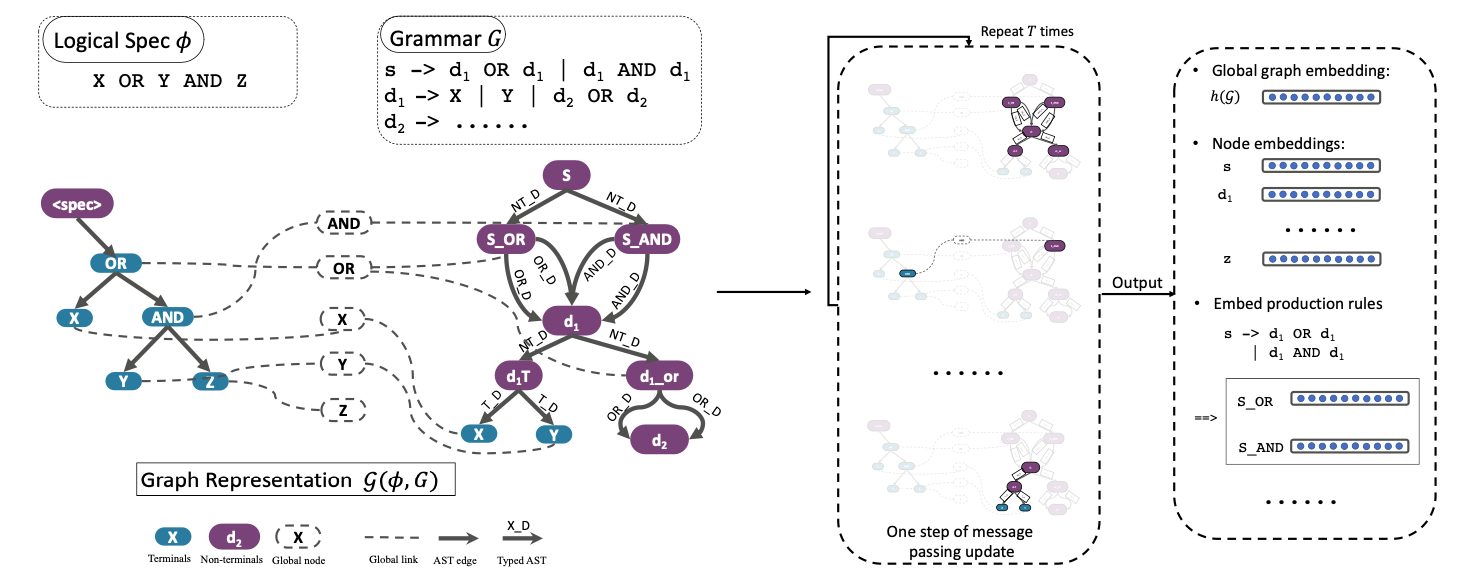
\includegraphics[width=\columnwidth]{Images/Synthesis1-1.png}}
\label{icml-historical}
\end{center}
\vskip -0.2in
\end{figure}
The Syntax-Guided Synthesis (SyGuS) problem is to synthesize a function f that satisfies two kinds of constraints:1) A syntactic constraint specified by a context-free grammar (CFG) G, and 2) A semantic constraint specified by a formula $\phi$ built from symbols in a background theory T along with f. The authors investigate how to efficiently synthesize the function f. Specifically, given a dataset of N tasks D = {($\phi_i$, G$_i$)}N$_i$=1, The following two tasks are addressed: 1) learning an algorithm A$_\theta$ : ($\phi$, G) $\rightarrow$ f parameterized by $\theta$ that can find the function f$_i$ for ($\phi_i$, G$_i$) $\in$ D; 2) given a new task set D$'$, adapt the above learned algorithm A$_\theta$ and execute it on new tasks in D$'$. This setting poses two difficulties in learning. First, the ground truth target function f is not readily available, making it difficult to formulate as a supervised learning problem. Second, the constraint $\varphi$ is typically verified using an SAT or SMT solver, and this solver in turns expects the generated f to be complete. This means the weak supervision signal will only be given after the entire program is generated. Thus, it is natural to formulate A$\theta$ as a reinforcement learning algorithm. Since each instance ($\phi_i$, G$_i$) $\in$ D is an independent task with different syntactic and semantic constraints, the key to success is the design of such meta-learner.
\subsubsection{Formal Definition}
\textbf{semantic spec $\varphi$} The spec itself is a program written using some grammar. The grammar used in spec $\varphi$ is different from the grammar G that specifies the syntax of the output program. However, in many practical cases the tokens (i.e., the dictionary of terminal symbols) may be shared across the input spec and the output program.

\textbf{CFG G} A context free grammar (CFG) is defined as G = ⟨V , E, R, s⟩. Here V denotes the non-terminal tokens, while E represents the terminal tokens. s is a special token that denotes the start of the language, and the language is generated according to the production rules defined in R. For a given non-terminal, the associated production rules can be written as $\alpha \rightarrow \beta_1 | \beta_2 .... | \beta_{n_\alpha}$, where ${n_\alpha}$ is the branching factor for non-terminal $\alpha \in V$, and $\beta _i$ = u$_1$u$_2$ . . . u$_{|\beta_i|} \in$  (V $\cup$ E). Each production rule $\alpha \rightarrow \beta_1 \in$ R represents a way of expanding the grammar tree, by attaching nodes u$_1$u$_2$ . . . u$_{|\beta_i|}$ to node $\alpha$.

\textbf{Output function f} The output is a program in the language generated by G. A valid output f must satisfy both the syntactic constraints specified by G and the semantic constraints specified by $\varphi$.
\subsubsection{Task Representation}
Semantic spec program $\varphi$ and the CFG G have rich structural information.To construct the graph, the abstract syntax tree (AST) is built first for the semantic spec program $\varphi$, according to its own grammar (typically different from the output grammar G). To represent the grammar G, each symbol in V $\rightarrow$ E with a node representation. Furthermore, for a non-terminal $\alpha$ and its corresponding production rules  $\alpha \rightarrow \beta_1 | \beta_2 .... | \beta_{n_\alpha}$, Additional nodes $\alpha_i$  are created for each substitute $\beta_i$. The purpose is to enable grammar adaptive program generation.

As a simplification, all nodes $\alpha_i$ is merged representing $\beta_i$ that is a single terminal token into one node. Finally, the global nodes for shared tokens in E are created to link together the shared variable and operator nodes. This enables information exchange between the syntactic and semantics specifications. To encode the joint graph G($\varphi$, G), graph neural networks is used to get the vector representation for each node in the graph. Specifically, for each node v $\in$ G, the following parameterization for one step of message passing style update:

\begin{math}
h^{(t+1)}_v = Aggregate({F(h^t_u , e_{u,v} )}_{u \in N(v)})
\end{math}

Lastly, {h$^t_v$}$_{v\in G}$ , h$^t_v \in r^d$ are the set of node embeddings. Here N (v) is the set of neighbor nodes of v, and $e_{u,v}$ denotes the type of edge that links the node u and v. F is parameterized as, F(h$^t$,e) = $\sigma$(W$^{eT}_t$h$^t$) where different matrices W$\in R^{dxd}$ are used for different edge types and different propagation steps t. All the node embeddings are aggregated to get the global graph embedding h(G). The embedding matrix for each non-terminal node is computed. Specifically, given node $\alpha$, the embedding matrix is H$_\alpha \in R^{n_\alpha x d}$, where the ith row of H$_\alpha^{(i)}$ is the embedding of node $\alpha_i$ that corresponds to substitution $\beta_i$.
\subsubsection{Grammar Adaptive Policy Network}
\begin{figure}[ht]
\vskip 0.2in
\begin{center}
\centerline{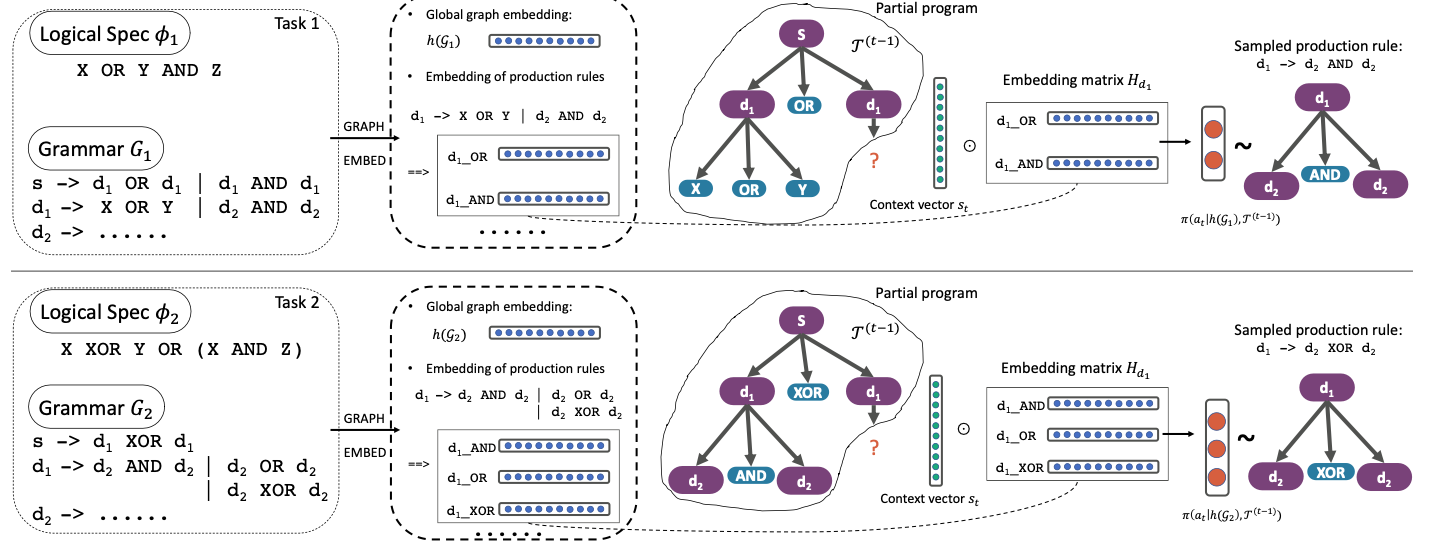
\includegraphics[width=\columnwidth]{Images/Synthesis1-2.png}}
\label{icml-historical}
\end{center}
\vskip -0.2in
\end{figure}

The key idea is to make the policy parameterized by decision embedding, rather than a fixed set of parameters. The embedding matrix H$_\alpha \in R^{n_\alpha x d}$ is used to perform decision for this time step. This allwos us to build  policy network in an auto-regressive way. Specifically, the policy $\pi(f|\phi,G)$ can be parameterized as:$\pi(f|\phi,G) = \prod_{t=1}^{|b|} \pi(a_t|h(G),T^{t-1}$, where $T^{t-1}= \alpha_1 ... \alpha_{t-1}$ denotes the partial tree. Here the probability of each action (in other words, each tree expansion decision) is defined as $\pi(a_t|h(G),T^{t-1}\propto exp(H_\alpha^{(i)T}s_t$, where $s_t \in R$ is the context vector that captures the state of h(G) and $T^{t-1}$. s$_t$ is tracked by a LSTM decoder whose hidden state is updated by the embedding of the chosen action h$_{alpha t}$ . The initial state s$_0$ is obtained by passing graph embedding h(G) through a dense layer with matching size.
\subsubsection{Solving Via Reinforced Learning}
let $\theta$ denote the parameters of graph embedding and adaptive policy network. For a given pair of instances ($\phi$, G), a learned policy $\pi_\theta(f|\phi,G)$ parameterized by $\theta$ that generates f such that $\phi\equiv$ f.

\textbf{Reward design} The RL episode starts by accepting the representation of tuple ⟨$\phi$, G⟩ as initial observation. During the episode, the model executes a sequence of actions to expand non-terminals in f, and finishes the episode when f is complete. Upon finishing, the SAT solver is invoked and will return a binary flag indicating whether f satisfies $\phi$ or not. To smooth the reward: for each specification $\phi$ the solution maintains a test case buffer B$_\phi$ that stores all input examples observed so far. Each time the SAT solver is invoked for $\phi$, if f passes then a full reward of 1 is given, otherwise the solver will generate a counter-example b besides the binary flag. Then sample interpolated examples around b which is denoted in the set as B$_b$. Then the reward is given as the fractions of examples in B$_\phi$ and B$_b$ where f has the equivalent output as $\phi$

\begin{math}
r = {\sum_{b=\in B_\phi\cup B_b} [f(b) \equiv \phi(b)]}/{|B_\phi\cup B_b|}
\end{math}

At the end of the episode, the buffer is updated as $B_\phi \leftarrow B_\phi\cup B_b$ for next time usage. The authors utilize the Advantage Actor-Critic (A2C) for model training. Given a training set D, a minibatch of instances are sampled from D for each epoch. For each instance$(\phi_i,G_i)$,the model performs a complete rollout using policy $\pi_\theta(f|\phi_i,G_i)$. The actor-critic method computes the gradients w.r.t to $\theta$ of each instance as

\begin{math}
d\theta \leftarrow \sum_{t=1}^{|f|} \bigtriangledown _\theta log\pi(\alpha_t|h(G),T^{(t)})(\gamma^{|f|-t}r-V(s_t;w)),
\end{math}

where $\gamma$ denotes the discounting factor and V (s$_t$; w) is a state value estimator parameterized by w. In implementation, this is modeled as a standard MLP with scalar output. It is learned to fit the expected return, i.e., min$_w E \sum _{t=1} ^{|f|} \gamma ^{-t}r-V(s_t;w)$ Gradients obtained from each instance are averaged over the minibatch before applying to the parameter.
\subsubsection{Results}
\begin{figure}[ht]
\vskip 0.2in
\begin{center}
\centerline{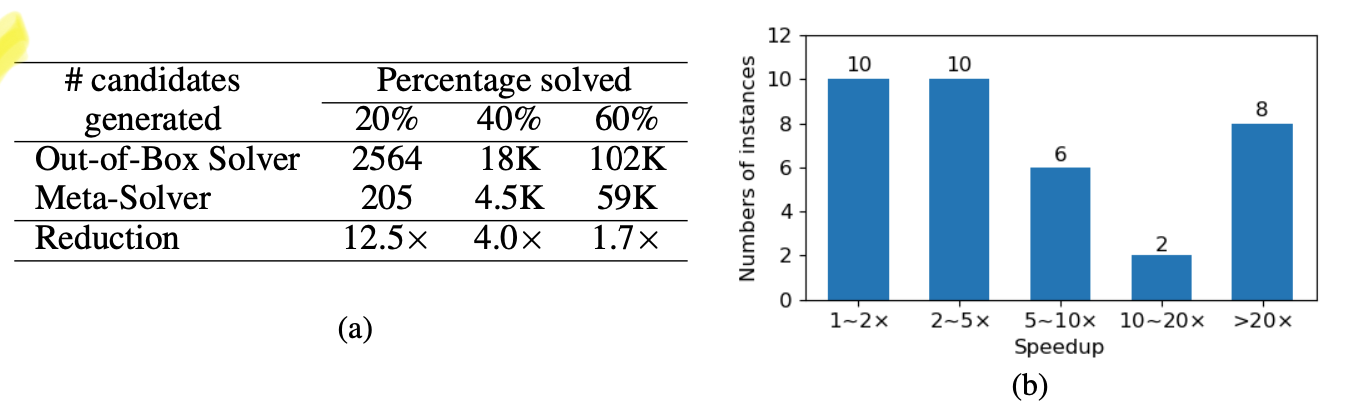
\includegraphics[width=\columnwidth]{Images/Synthesis1-3.png}}
\label{icml-historical}
\end{center}
\vskip -0.2in
\end{figure}
Performance improvement with meta-learning. (a) Accumulated number of candidates generated in order to solve 20 percent, 40 percent, and 60 percent of the testing tasks; and (b) speedup distribution over individual instances.
\subsection{ExprGen}
\subsubsection{Background}
The most general form of the code generation task is to produce a (partial) program in a programming language given some context information c. This context information can be natural language (as in, e.g., semantic parsing), input-output examples (e.g., inductive program synthesis), partial program sketches. The key idea is to construct the AST a sequentially, by expanding one node at a time using production rules from the underlying programming language grammar.  Then, the probability of generating a given AST a given some context c is

\begin{math}
p(a|c) = \prod_t p(a_t|c,a_{<t})
\end{math}

where a$_t$ is the production choice at step t and a<t the partial syntax tree generated before step t.

\textbf{Code Generation as Hole Completion} the authors introduce the ExprGen task of filling in code within a hole of an otherwise existing program. They assume information about the following code as well and aim to generate whole expressions rather than single tokens. They restrict themselves to expressions that have Boolean, arithmetic or string type, or arrays of such types.
\subsubsection{Graph Decoding for source code}
Tasks include to encode the code context c, $v_1, . . . , v_l$ and to construct a model that can learn p$(a_t | c,a_{<t})$ well. Both these encoders yield a distributed vector representation for the overall context, representations $h_{t_1} , . . . , h_{t_T}$ for all tokens in the context, and separate representations for each of the in-scope variables $v_1, . . . , v_l$, summarizing how each variable is used in the context. The decoder model follows the grammar-driven AST generation strategy is used. A variation of attribute grammars (Knuth, 1967) from compiler theory to derive the structure of this graph. Each node in the AST is associated with two fresh nodes representing inherited resp. synthesized information (or attributes). Inherited information is derived from the context and parts of the AST that are already generated, whereas synthesized information can be viewed as a “summary” of a subtree. In classical compiler theory, inherited attributes usually contain information such as declared variables and their types (to allow the compiler to check that only declared variables are used), whereas synthesized attributes carry information about a subtree “to the right” (e.g., which variables have been declared). Traditionally, to implement this, the language grammar has to be extended with explicit rules for deriving and synthesizing attributes. Attributes are represented by distributed vector representations and train neural networks to learn how to compute attributes. A deterministic procedure that turns a partial AST a$_{<t}$ into a graph by adding additional edges that encode attribute relationships, and a graph neural network that learns from this graph.

\begin{figure}[ht]
\vskip 0.2in
\begin{center}
\centerline{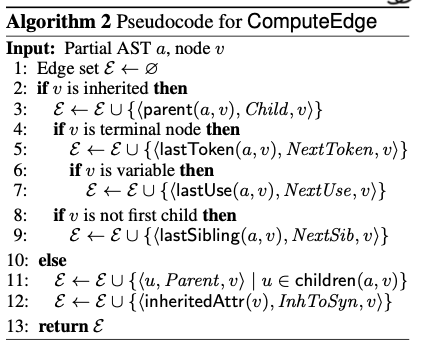
\includegraphics[width=\columnwidth]{Images/Synthesis2-1.png}}
\label{icml-historical}
\end{center}
\vskip -0.2in
\end{figure}
\begin{figure}[ht]
\vskip 0.2in
\begin{center}
\centerline{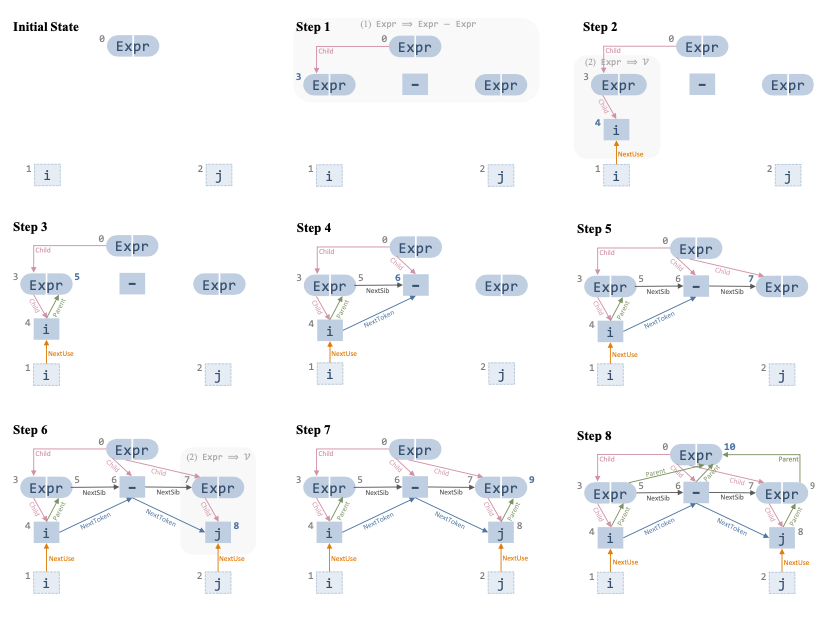
\includegraphics[width=\columnwidth]{Images/Synthesis2-2.png}}
\label{icml-historical}
\end{center}
\vskip -0.2in
\end{figure}

\textbf{Notion} as graphs where nodes u, v, . . . are either the AST nodes or their associated attribute nodes, and typed directed edges ⟨u, $\tau$, v⟩ $\in$ E connect the nodes according to the flow of information in the model. The edge types $\tau$ represent different syntactic or semantic relations in the information flow. E$_v$ is defined as a set of incoming edges into v. They also use functions like parent(a, v) and lastSibling(a, v) that look up and return nodes from the AST a (e.g. resp. the parent node of v or the preceding AST sibling of v) expanded to the set of known variables using the production rule (2) : Expr $\implies$ V, choosing i for the first variable and j for the second variable.

\textbf{Edges in a$_{<t}$} - Child (red) edges connect an inherited attribute node to the inherited attributes nodes of its children, as seen in the edges from node 0. Parent (green) edges connect a synthesized attribute node to the synthesized attribute node of its AST parent, as seen in the edges leading to node 10. These are the additional connections used by the R3NN decoder. NextSib(black) edges connect the synthesized attribute node to the inherited attribute node of its next sibling (e.g. from node 5 to node 6). These allow information about the synthesized attribute nodes from a fully generated subtree to flow to the next subtree. NextUse (orange) edges connect the attribute nodes of a variable (since variables are always terminal nodes, the posposed solution does not distinguish inherited from synthesized attributes) to their next use. They just follow the lexical order. NextToken (blue) edges connect a terminal node (a token) to the next token in the program text, for example between nodes 4 and 6. InhToSyn edges (not shown in Fig) connect the inherited attributes nodes to its synthesized attribute nodes. This is not strictly adding any information, but was found helpful with training.

\textbf{Attribute Node Representations} To compute the neural attribute representation h$_v$ of an attribute node v whose corresponding AST node is labeled with l$_v$, incoming edges are obtained and then use the state update function from Gated Graph Neural Networks (GGNN). The attribute representations h$_{u_i}$ at edge sources u$_i$ is used to transform them according to the corresponding edge type t$_i$ using a learned function f$_{t_i}$. They are aggregated (by elementwise summation) and combine them with the learned embedding emb(l$_v$) of the node label l$_v$ using a function g:

\begin{math}
h_v = g(emb(l_v), \sum_{<u_i,t_i,v>\in E_v} f_{t_i} (h_{u_i}))
\end{math}

The authors use a single linear layer for $f_{t_i}$ and implement g as a gated recurrent unit. Node representations is computed in such an order that all h$_{u_i}$ appearing on the right are already computed.

\textbf{Choosing Productions, Variables \& Literal} For a nonterminal node v with label l$_v$ and inherited attributes h$_v$, pickProduction(l$_v$,h$_v$) = argmax P(rule |l$_v$,h$_v$) = argmax[e(h$_v$)+m$_{l_v}$]. (3) Here, m$_{l_v}$ is a mask vector whose value is 0 for valid productions l$_v \implies ...$ and $-\infty$for all other productions. In practice, e is implemented using a linear layer. Similarly, variables are picked from the set of variables V in scope using their representations h$_{v_{var}}$ (initially the representation obtained from the context, and later the attribute representation of the last node in the graph in which they have been used) by using a pointer network. Concretely, to pick a variable at node v, learnable linear function k is used and define pickVariable(V,h$_v$) = argmax$_{var \in V}$ P(var|h$_v$) = argmax$_{var \in V}$k(h$_v$,h$_{v_{var}}$ )(4) Note that since the model always picks a variable from the set of in-scope variables V , this generation model can never predict an unknown or out-of-scope variable. They combine a small vocabulary L of common literals observed in the training data and special UNK tokens for each type of literal with another pointer network that can copy one of the tokens $t_1...t_T$ from the context.Thus,to pick a literal at node v, and define pickLiteral(V,h$_v$) = argmax$_{lit\in L \cup {t_1...t_T}}$ P(lit|h$_v$)(5). This is implemented by learning two functions s$_L$ and s$_c$, such that s$_L$(h$_v$) produces a score for each token from the vocabulary and s$_c$ (h$_v$ , h$_{t_i}$ ) computes a score for copying token t$_i$ from the context. By computing a softmax over all resulting values and normalizing it by summing up entries corresponding to the same constant, they can learn to approximate the desired P (lit | h$_v$ )

\textbf{Training \& Training Objective} note that given a ground truth target tree, one can easily augment it with all additional edges. Given that full graph, one can compute a propagation schedule (intuitively, a topological ordering of the nodes in the graph, starting in the root node) that allows to repeatedly apply (2) to obtain representations for all nodes in the graph. By representing a batch of graphs as one large (sparse) graph with many disconnected components,

\textbf{Additional Improvements} (3) is extended with an attention mechanism that uses the state h$_v$ of the currently expanded node v as a key and the context token representations $h_{t_1} , . . . , h_{t_T}$ as memories. Experimentally, it was found that extending Eqs. 4, 5 similarly did not improve results, probably due to the fact that they already are highly dependent on the context information. Additional information for Child edges is porivded. To allow this, the setup is changed so that some edge types also require an additional label, which is used when computing the messages sent between different nodes in the graph. Concretely, (2) is extended by considering sets of unlabeled edges E$_v$ and labeled edges E$_v^l$:

\begin{math}
h_v = g(emb(l_v), \sum_{<u_i,t_i,v>\in E_v} f_{t_i} (h_{u_i}) + \sum_{<u_i,t_i,l_i,v>\in E_v^l} f_{t_i} (h_{u_i},emb_e(l_i)))
\end{math}

Thus for labeled edge types, f$_{t_i}$ takes two inputs and a learnable embedding for the edge labels. The authors found it useful to label Child with tuples consisting of the chosen production and the index of the child, they would label the edge from 0 to 3 with (2,0), the edge from 0 to 6 with (2,1), etc. the model was extended pickProduction to also take the information about available variables into account. Intuitively, this is useful in cases of productions such as Expr $\implies$ Expr.Length, which can only be used in a well-typed derivation if an array-typed variable is available. Thus, e(h$_v$) is extended from (3) to additionally take the representation of all variables in scope into account, i.e., e(h$_v,r({h_{v_var} | var \in V}))$, where r is a max pooling operation.
\subsubsection{Results}
\begin{figure}[ht]
\vskip 0.2in
\begin{center}
\centerline{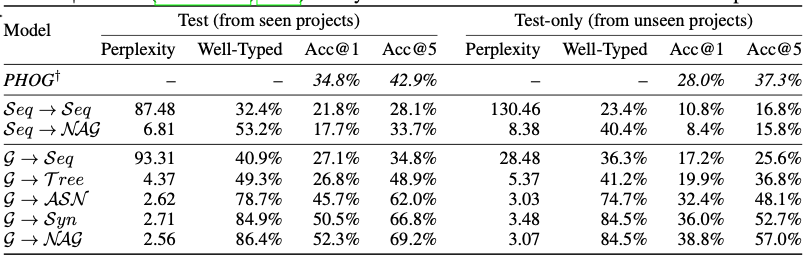
\includegraphics[width=\columnwidth]{Images/Synthesis2-3.png}}
\label{icml-historical}
\end{center}
\vskip -0.2in
\end{figure}
Evaluation of encoder and decoder combinations on predicting an expression from code context.PHOG (Bielik et al., 2016) is only conditioned on the tokens on the left of the expression
\subsection{AutoPandas}
\subsubsection{Technique}
\textbf{Generators} The authors first formally describe generators. In their setting, a generator G is a program that, when invoked, outputs values from a space of possible values.their generators G can contain arbitrary Python code, along with a set of stateful operators that govern the behavior of G across runs. An example of such an operator is Select.
\begin{figure}[ht]
\vskip 0.2in
\begin{center}
\centerline{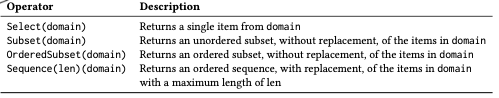
\includegraphics[width=\columnwidth]{Images/Synthesis3-1.png}}
\label{icml-historical}
\end{center}
\vskip -0.2in
\end{figure}
\textbf{Operators} Apart from Select, three other operators are supported, namely (1) Subset, (2) OrderedSubset and (3) Sequence. An informal description of their behavior is provided in Table above. The behavior of the generator across runs can be controlled by changing the semantics of these operators. 
Randomized: The simplest case is for the generator to be randomized.
Exhaustive (Depth-First). Another option is to have an exhaustive generator which systematically explores all possible execution paths as governed by the constituent operator calls. 
The operator semantics uses three internal state variables t , $\sigma$ and $\delta$ . The variable t keeps track of the number of operator calls made in the current invocation of the generator. The variable $\sigma$ is a map from the operator call index to the choice to be made by the operator call in the current invocation of the generator. $\delta$ represents a map from the operator call index to the collection of possible values W as defined by the operator type and the passed domain D. The variables $\sigma$ and $\delta$ are initialized to empty maps before the first invocation of the generator, but are persisted across the later ones. However t is reset to zero before every fresh generator invocation. A special operator is introduced called Op End that is implicitly invoked at the end of each invocation in the generator. Then the authors now briefly explain the rationale behind all of these variables, Op End and the rules themselves.
(1) Op-Extend - This rule governs the behavior of the operator when it is invoked for the first time (as signified by t $\notin$ dom($\sigma$ )). The operator returns the first value from W and records this choice in $\sigma$  . It also stores W in  $\delta$ for future use.
(2) Op-Replay - The hypothesis t $\in$ dom($\sigma$  ) signifies that this operator call needs to replay the choice as dictated by $\sigma$ (t ).
(3) Op-End-1 - This rule captures the first behavior of the special operator Op End. It finds the last (deepest) operator call, indexed by k , that has not exhausted all possibilities, and increments its entry in $\sigma$  . This is key to enforcing depth-first semantics - a later call explores all possibilities before previous calls do the same. Note that it also pops-off the later entries (> k) from $\sigma$  and $\delta$. This is required as the generator may take an entirely new path based on the new value returned by this operator and may therefore make an entirely new set of operator calls. Together, these two steps maintain the invariant that $\sigma$  stores the choice to be made by the operators in the current generator run.
(4) Op-End-2 - The final rule covers the case when all operator calls have exhausted all possible values. This makes the special Op End operator signal Generator-Exhausted after the last invocation of the generator, indicating that they authors have explored all possible executions of the generator.

\begin{figure}[ht]
\vskip 0.2in
\begin{center}
\centerline{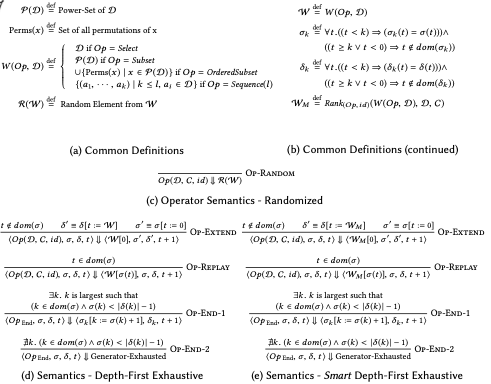
\includegraphics[width=\columnwidth]{Images/Synthesis3-2.png}}
\label{icml-historical}
\end{center}
\vskip -0.2in
\end{figure}

\textbf{Generator-Based Program Synthesis} To build an enumerative synthesis engine E using generators.The engine consists of two components D(1) a program candidate generator and (2) a checker that checks if the candidate program produces the correct output. Program Candidate Generator. A program candidate generator P is a generator that, given an input-output example, generates program candidates.

\textbf{Building an Exhaustive Depth-First Enumerative Synthesis Engine} Using the exhaustive depth-first semantics for operators presented in figure above for the generator gives an exhaustive depth-first synthesis engine. 

\textbf{Building a Smart Enumerative Synthesis Engine} The generator in figure above describes a space of programs that is extremely large for such an enumerative pandas synthesis engine to explore in reasonable time.

\textbf{Neural-Network Query} The query Q to each neural network model, regardless of the operator, is of the form Q = (D, C) where D and C are the domain and context passed to the operator.

\textbf{Query Encoding} Encoding this query into a neural-network suitable format poses several challenges. Recall that the context and the domain passed to operators in the pandas program candidate generator contain complex structures such as dataframes. Dataframes are 2-D structures which can contain arbitrary Python objects as primitive elements. Even restricting to strings or numbers, the set of possible primitive elements is infinite. This renders all common value-to-value map-based encoding techniques popular in machine learning, such as one-hot encoding, inapplicable. At the same time, the encoding needs to retain enough information about the context to generalize to unseen queries which may occur when the synthesis engine is deployed in practice. Therefore, simply abstracting away the exact values is not viable. In summary, a suitable encoding needs to (1) abstract away only irrelevant information and (2) be suitably structured for neural processing. a graph-based encoding was designed that possesses all these desirable properties.

\textbf{Graph-Based Encoding} the authors describe how to encode the domain D and the context C as a graph, consisting of nodes, edges between pairs of nodes, and labels on nodes and edges. The overall rationale is that it is not the concrete values, but rather the relationships amongst values, that really encode the transformation at hand. That is, relationship edges should be sufficient for a neural network to learn from. For example, the essence of transformation is that the values of the column ‘Category’ now become the columns of the pivoted dataframe, with the ‘Date’ column as an index, and the ‘Expense’ as values. The concrete names are immaterial.
Recall that the domain and context are essentially collections of elements. How to encode each such element e individually as a graph Ge is described below. followed by the description of the procedure to combine these graphs into a single graph G Q representing the graph-encoding of the full query Q.

\textbf{Encoding Primitives} If the element e is a primitive value (strings, ints, float, lambda, NaN etc.), its graph encoding Ge contains a single node representing e. This node is assigned a label based on the data-type of the element as well as the source of the element. The source of an element indicates whether it is part of the domain, if it is one of the input-outputs in the I/O example, if it is one of the intermediates, or none of these.

\textbf{Encoding DataFrames} If the element e is a dataframe, each cell element in the dataframe is encoded as a node in the graph Ge . The label of the node includes the type of the element (string, number, float, lambda, NaN, etc.). The label also includes the source of the dataframe, i.e. whether the dataframe is part of the domain, input, output, intermediate, or none of these. Nodes are added to Ge that represent the schema of the dataframe, by creating a node for each row index and column name of the dataframe. Finally, a representor node is added to Ge that represents the whole of the dataframe. The label of this node contains the type (dataframe) as well as the source of the parent dataframe. Note that this additional representor node is not created when encoding primitive elements. The node representing the primitive element itself acts as its representor node. The graph encoding of a dataframe also contains three kinds of edges to retain the structure of the dataframe. The first kind is adjacency edges. These are added between each pair of cell nodes, column name nodes or row index nodes that are adjacent to each other in the dataframe. Adjacency edges in the four cardinal directions only. The second kind is indexing edges, which are added between each column name node (resp. row index node) and all the cell nodes that belong to that column (resp. row). Finally, the third kind of edge is a representation edge, between the representor node to all the other nodes corresponding to the contents of the dataframe.

\textbf{Encoding the Query Q} To encode Q = (D, C), G$_e$ is constructed for each element in D and C as described above, and create a graph G containing these G$_e$ s as sub-graphs. Additionally, to capture relationships amongst these elements, a fourth kind of edge is added - the equality edge, between nodes originating in different G$_e$s such that the elements they represent are equal. Formally, an equality edge between nodes n$_1$ and n$_2$ is added if n$_1 \in G_{e_i} \wedge n_2 \in G_{e_j} \wedge i\neq j \wedge$V(n$_1$)=V(n$_2$) where V is a function that given n, retrieves the value encoded as n. For representor nodes, V returns the whole element it represents. For example, for a dataframe, V would return the dataframe itself for the representor node. Equality edges are key to capturing relationships between the inputs and the output in the I/O example, as well as the domain D and the I/O example. The neural network model can then learn to extract these relationships and use them to infer the required probability distribution.

\textbf{Operator-Specific Graph Neural Network Models} Given the graph-based encoding G$_Q$ of a query Q, itis fed to a graph neural network model. Each operator has a different model. The input to all network models is a undirected graph G = (V, E, X). V and X characterize the nodes, where V is the set of nodes and X is the embedding X : V $\rightarrow R^D$. Effectively, X maps each node to a one-hot encoding of its label of size D, where D is a hyper-parameter. E contains the edges,where each edge $e\in E $ is a 3-tuple(v$_s$,v$_t$,t$_e$). The source and target nodes are v$_s$ and v$_t$, respectively. The type t$_e$ of the edge is one of $\Gamma _e \equiv$ {adjacency, indexing, representor, equality} and is also one-hot encoded. Each node v is assigned as t at e vector h$_v \in R^D$ . The vector to the node embedding h(0) = X(v) is initialized. The network then propagates information via r rounds of message passing. During round k (0 $\leq$ k < r ), messages are sent across edges. In particular, for each edge (v$_s$,v$_t$,t$_e$), v$_s$ sends the message $m_{v_s \rightarrow v_t} = f_k(h^{(k)}_{v_s},t_e )$ to $v_t$. $f_k : R^{D+|\tau_e|} → R^D$ is a single linear layer. These are parameterized by a weight matrix and a bias vector, which are learnable parameters. Each node v aggregates its incoming messages into $m_{v} = g({m_{v_s \rightarrow v}|(v_s,v,t_e) \in E})$ using the aggregator g. the authors take g to be the element-wise mean of the incoming messages. The new node state vector h$^{(k+1)}_v$ for the next round is then computed as h$^{(k+1)}_v$ = GRU(m$_v$ ,h$^{(k)}_v$) where GRU is the gated recurrent unit [Cho et al. 2014] with start state as h$^{(k)}_v$ and input m . r = 3 rounds of message passing, as experimentally noticed that further increasing the number of message passing rounds did not increase validation accuracy. After message passing is completed, they have the updated state vectors h$^{(r)}_v$ for each node v. Now depending on the operator, these node vectors are further processed in different ways as described below to obtain the corresponding probability distributions over space of values defined by the operator.

\textbf{Select} Element-wise sum-pooling of the node state vectors is performed h$^{(r)}_v$ into a graph state vector h$_G$ . Followed by concatenation of h$_G$ with the node state vectors h$^{(r)}_{di}$ of the representor nodes di for di each element in the domain D in the query Q, to obtain vectors h$_i$ = h$_G$ * h$^{(r)}_{di}$. h$_{i_s}$ is passed though a multi-layer perceptron with one hidden layer and a one-dimensional output layer, and apply softmax over the output values for all the elements to produce a probability distribution over the domain elements ($p_1,··· ,p_n$). For inference,this distribution is returned as the result,while during training they compute cross-entropy loss w.r.t this distribution and the correct distribution where p$_i$ = 1 for the correct choice i and $\forall j \neq i, p_j = 0$.

\textbf{Subset} As in Select, element-wise sum-pooling of the node state vectors is performed and concatenate it with the state vectors of representor nodes to obtain the vectors h$_i$ = h$_G$ * h$^{(r)}_{di}$ for each element in the domain. However, the h$_{i_s}$ is passed though a multi-layer perceptron with one hidden layer and apply softmax activation on the output layer to obtain a distribution (p$_{i_k}$ ,p$_{e_k}$ ) over two label classes "include" and "exclude" for each of the domain element d$_k$ individually. Recall that the space of possible outputs for the Subset operator is the power-set of the domain D. The probability of these labels corresponds to the probability with which an element is included and excluded from the output set respectively. To compute the probability distribution, the probability of each possible output set is computed as simply the product of the "include" probabilities for the elements included in the set and the "exclude" probabilities for the elements excluded from the set. Again, this distribution is returned as the result during inference, while during training, loss is computed w.r.t this distribution and the correct individual distribution of the elements where p$_{i_k} = 1 \wedge $ p$_{e_k}$ =0 if element d$_k$ is present in the correct output,else p$_{i_k} = 0 \wedge $ p$_{e_k}$ =1.

\textbf{OrderedSubset and Sequence} element-wise sum-pooling of the node state vectors h$^{(r)}_v$ is performed into a graph state vector h$_G$. h$_G$ is passed to an LSTM that is unrolled for T + 1 time-steps, vGG where T = $|D|$ for OrderedSubset and T = l for Sequence(l) where l the max-length parameter passed to Sequence. The extra time-step is to accommodate a terminal token. For each time-step t, the output ot is concatenated with the node state vectors h$^{(r)}_{di}$ of the representor nodes d$_{i_s}$ for each element in the domain passed to the operator to obtain vectors h$_i^t$ = o$_t$ * h$^{(r)}_{di}$. At time-step t, in a similar fashion as Select, a probability distribution is then computed over the domain elements plus an arbitrary terminal token term. The terminal token is used to indicate the end of a sequence/set. Now, to compute the probability distribution, the probability of each set or sequence ($a_0, · · · , a_k$ ) where (k $\leq$ T ) is simply the product of probabilities of a$_i$ at time-step i and the probability of the terminal token term at time-step k + 1. As before, this distribution is directly returned during inference, while during training, loss is aggregated over individual time-steps; the loss for a time-step is computed as described in Select. All the network models are trained with the ADAM optimizer  using cross-entropy loss.

\textbf{Training Neural-Backed Generators for Pandas} Tuples of the form (I, O, P, K) where P is a pandas program such that P(I) = O i.e. it produces O when executed on inputs I. Also, K is the sequence of choices made by the operators in the generator such that the generator produces the program P when it is fed I and O as inputs. Then, it is straight-forward to extract training data tuples (C, D,c) for each operator call by simply running the generator on I and O and recording the concrete context C and domain D passed to the operator, and forcing the operator to make the choice c. These tuples are also meaningful by construction, as the operators make choices that lead to the generation of the program P which solves the synthesis task described by I and O. The second insight is that one can obtain these (I, O, P, K) tuples by using the generator itself. After generating random inputs I (DataFrames), run the generator on I using the randomized semantics while simultaneously recording the choices made as K. The program P returned by the generator is then run on I to yield O.

\subsubsection{Results}
\begin{figure}[ht]
\vskip 0.2in
\begin{center}
\centerline{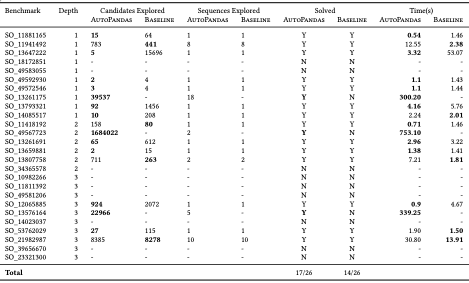
\includegraphics[width=\columnwidth]{Images/Synthesis3-3.png}}
\label{icml-historical}
\end{center}
\vskip -0.2in
\end{figure}
Performance on Real-World Benchmarks. Dashes (-) indicate timeouts by the technique. The code is published at https://github.com/rbavishi/autopandas.

\section{Bug Detection}
\subsection{Introduction}
Graph-structured data appears frequently in domains including chemistry, natural language semantics, social networks, and knowledge bases. In part of this survey, they study feature learning techniques for graph-structured inputs. Starting point is previous work on Graph Neural Networks, which the authors modify to use gated recurrent units and modern optimization techniques and then extend to output sequences. The result is a flexible and broadly useful class of neural network models that has favorable inductive biases relative to purely sequence-based models (e.g., LSTMs) when the problem is graph-structured.

Another paper presents an alternative approach to creating static bug finders. Instead of relying on human expertise, they utilize deep neural networks to train static analyzers directly from data. In particular, they frame the problem of bug finding as a classification task and train a classifier to differentiate the buggy from non-buggy programs using Graph Neural Network (GNN). Static analysis is an effective technique to catch bugs early when they are cheap to fix. Unlike dynamic analysis, static analysis reasons about every path in a program, offering formal guarantees for its run-time behavior. As an evidence of their increasing maturity and popularity, many static analyzers have been adopted by major tech companies to prevent bugs leaked to their production code. Examples include Google’s Tricorder, Facebook’s Getafix and Zoncolan, and Microsoft’s Visual Studio IntelliCode.

Despite the significant progress, static analyzers suffer from several well-known issues. One, in particular, is the high false positive rate which tends to overshadow true positives and hurt usability. The reason for this phenomenon is well-known: all nontrivial program properties are mathematically undecidable, meaning that automated reasoning of software generally must involve approximation. On the other hand, problems of false negatives also need to be dealt with. Recently, Habib and Pradel investigated how effective the state-of-the-art static analyzers are in handling a set of real-world bugs. Habib et al. show more than 90 percent of the bugs are missed, exposing the severity of false negatives.

Software defect prediction, which predicts defective code regions, can help developers find bugs and prioritize their testing efforts. To build accurate prediction models, previous studies focus on manually designing features that encode the characteristics of programs and exploring different machine learning algorithms. Existing traditional features often fail to capture the semantic differences of programs, and such a capability is needed for building accurate prediction models.
\subsection{Related work}

The most closely related work is GNNs. \cite{Micheli2009} proposed another closely related model that differs from GNNs mainly in the output model. GNNs have many of the same desirable properties of pointer networks (\cite{vinyals2017pointer}); when using node selection output layers, nodes from the input can be chosen as outputs. There are two main differences: first, in GNNs the graph structure is explicit, which makes the models less general but may provide stronger generalization ability; second, pointer networks require that each node has properties (e.g., a location in space), while GNNs can represent nodes that are defined only by their position in the graph, which makes them more general along a different dimension.
GGS-NNs are related to soft alignment and attentional models (e.g., \cite{bahdanau2016neural}; \cite{kumar2016ask}; \cite{sukhbaatar2015endtoend}) in two respects: first, the graph representation uses context to focus attention on which nodes are important to the current decision; second, node annotations in the program verification example keep track of which nodes have been explained so far, which gives an explicit mechanism for making sure that each node in the input has been used over the sequence of producing an output.  

\subsection{Gated Graph Sequence Neural Networks}
This paper's main contribution is an extension of Graph Neural Networks that outputs sequences. Previous work on feature learning for graph-structured inputs has focused on models that produce single outputs such as graph-level classifications, but many problems with graph inputs require outputting sequences. There are two settings for feature learning on graphs: (1) learning a representation of the input graph, and (2) learning representations of the internal state during the process of producing a sequence of outputs. The implementation is published at https://github.com/yujiali/ggnn.
\subsubsection{Graph Representation- GNN and GATED}
GNNs are a general neural network architecture defined according to a graph structure G = (V,E). Nodes v $\in$ V take unique values from 1, . . . , $|V|$, and edges are pairs e = (v, v$'$) $\in$ V × V. The authors focus in this work on directed graphs, so (v, v$'$) represents a directed edge v $\rightarrow$ v$'$, but note that the framework can easily be adapted to undirected graphs; see \cite{10.1109/TNN.2008.2005605}. The node vector (or node representation or node embedding) for node v is denoted by h$_v \in R^D$. Graphs may also contain node labels l$_v \in$ {1,...,L$_V$} for each node v and edge labels or edge types l$_e \in$ {1,...,L$_E$} for each edge. They overload notation and let h$_S$ = {h$_v | v \in S$} when S is a set of nodes, and l$_S$ = {l$_e | e \in S$} when S is a set of edges. The function IN(v) = {v$'$ |(v$'$,v) $\in$ E} returns the set of predecessor nodes v$'$ with v$'$ $\rightarrow$v. Analogously, OUT(v) = {v$'$ | (v, v$'$) $\in$ E} is the set of successor nodes v$'$ with edges v $\rightarrow$ v$'$. The set of all nodes neighboring v is NBR(v) = IN(v) $\cup$ OUT(v), and the set of all edges incoming to or outgoing from v is CO(v)={(v$'$,v$''$)$\in$E$|$v=v$'$Vv=v$''$}.GNNs map graphs to outputs via two steps. First, there is a propagation step that computes node representations for each node; second,an output model o$_v$ =g(h$_v$,l$_v$) maps from node representations and corresponding labels to an output o$_v$ for each v $\in$ V. In the notation for g, they leave the dependence on parameters implicit.

In GNNs, there is no point in initializing node representations because the contraction map constraint ensures that the fixed point is independent of the initializations. This is no longer the case with GG-NNs, which lets the authors to incorporate node labels as additional inputs. To distinguish these node labels used as inputs from the ones introduced before, called node annotations, and use vector x to denote these annotations. This will cause the first dimension of node representation to be copied along forward edges. With this setting of parameters, the propagation step will cause all nodes reachable from s to have their first bit of node representation set to 1. The output step classifier can then easily tell whether node t is reachable from s by looking whether some node has nonzero entries in the first two dimensions of its representation vector.
\subsubsection{Propogation Model- GNN and GATED}
An iterative procedure propagates node representations. Initial node representations h$_v$ are set to arbitrary values, then each node representation is updated following the recurrence below until convergence, where t denotes the timestep:

\begin{math}
h_v^{(t)} = f^\ast(l_v,l_{Co(v)},l_{NBR(v)}, h^{t-1}_{NBR(v)})
\end{math}

Several variants are discussed in \cite{10.1109/TNN.2008.2005605} including positional graph forms, node-specific updates, and alternative representations of neighborhoods. Concretely, \cite{10.1109/TNN.2008.2005605} suggest decomposing f$_\ast(\dot)$ to be a sum of per-edge terms.

\begin{figure}[ht]
\vskip 0.2in
\begin{center}
\centerline{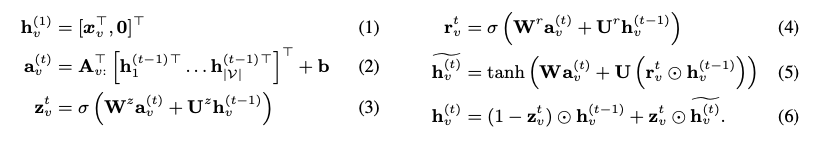
\includegraphics[width=\columnwidth]{Images/Bug1-1.png}}
\label{icml-historical}
\end{center}
\vskip -0.2in
\end{figure}

\begin{figure}[ht]
\vskip 0.2in
\begin{center}
\centerline{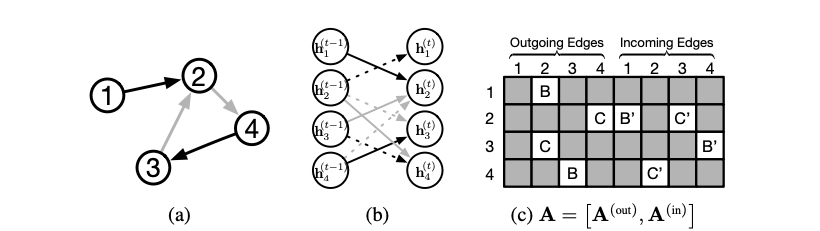
\includegraphics[width=\columnwidth]{Images/Bug1-2.png}}
\label{icml-historical}
\end{center}
\vskip -0.2in
\end{figure}

The matrix A $\in R^{D|V|x2D|V|}$ determines how nodes in the graph communicate with each other. The sparsity structure and parameter tying in A is illustrated in Figure above. The sparsity structure corresponds to the edges of the graph, and the parameters in each submatrix are determined by the edge type and direction. A$_v \in R^{D|V|x2D|V|}$ are the two columns of blocks in A(out) and A(in) corresponding to node v. Eq. 1 is the initialization step, which copies node annotations into the first components of the hidden state and pads the rest with zeros. Eq. 2 is the step that passes information between different nodes of the graph via incoming and outgoing edges with parameters dependent on the edge type and direction. Contains activations from edges in both directions. The remaining are GRU-like updates that incorporate information from the other nodes and from the previous timestep to update each node’s hidden state. z and r are the update and reset gates, $\sigma(x) = 1/(1+e^{-x}$ is the logistic sigmoid function, and multiplication is element-wise multiplication. Initial experiments with a vanilla recurrent neural network-style update, but in preliminary experiments found this GRU-like propagation step to be more effective.
\subsubsection{Output Model and Learning- GNN and Gated}
The output model is defined per node and is a differentiable function g(h$_v$ , l$_v$ ) that maps to an output. This is generally a linear or neural network mapping.independent per node, which are implemented by mapping the final node representations h$_v^{(T)}$ , to an output o$_v$ = g(h$_v$ ,l$_v$) for each node v $\in$ V. To handle graph-level classifications. Learning is done via the Almeida-Pineda algorithm, which works by running the propagation to convergence, and then computing gradients based upon the converged solution. This has the advantage of not needing to store intermediate states in order to compute gradients. The disadvantage is that parameters must be constrained so that the propagation step is a contraction map.

GG-NNs support node selection tasks by making o$_v$ = g(h$_v$ , x$_v$ ) for each node v $\in$ V output node scores and applying a softmax over node scores. Second, for graph-level outputs, a graph level representation vector is defined as

\begin{math}
h_G = tanh(\sum_{v \in V} \sigma(i(h_v^{(T)},x_v))X(tanh(j(h_v^{(T)},x_v))))
\end{math}

where $\sigma(i(h_v^{(T)},x_v))$ acts as a soft attention mechanism that decides which nodes are relevant to the current graph-level task. i and j are neural networks that take the concatenation of h$_v^{(T)}$ and x$_v$ as input and outputs real-valued vectors.
\subsubsection{Gated Graph Sequence Neural Networks}
several GG-NNs operate in sequence to produce an output sequence $o^{(1)} . . . o^{(K )}$. For the k$^{th}$ output step, the matrix of node annotations is denoted as $X^{(k)} = [x_1^{(k)}; . . . ; x_{|V|}^{(k)}]^T \in R^{|V|×L_V}$. Two GG-NNs are used: F$_o^{(k)}$ and F$_x^{(k)}$: F$_o^{(k)}$ for predicting o$^{(k)}$ from X$^{(k)}$, and F$^{(k)}_x$ for predicting X$^{(k+1)}$ from X$^{(k)}$. X$^{(k+1)}$ can be seen as the states carried over from step k to k + 1. Both F$_o^{(k)}$ and F$_x^{(k)}$ contain a propagation model and an output model. In the propagation models, the matrix of node vectors  at the t$^{th}$ propagation step of the k$^{th}$ output step is denoted as H$^{(k,t)} = [h_1^{(k,t)};...;h_{|V|}^{(k,t)}]^T \in R^{|V|×D}$. As before, in step k, H$^{(k,t)}$ is set by 0-extending X$^{(k)}$ per node. Alternatively, F$_o^{(k)}$ and F$_x^{(k)}$ can share a single propagation model, and just have separate output models. This simpler variant is faster to train and evaluate, and in many cases can achieve similar performance level as the full model. But in cases where the desired propagation behavior for F$_o^{(k)}$ and F$_x^{(k)}$ are different, this variant may not work as well.

A node annotation output model for predicting X$^{(k+1)}$ from H$^{(k,T)}$ is introduced. The prediction is done for each node independently using a neural network $j(h_v^{(T)},x_v)$ of h$_v$ and x$_v$ as input and outputs a vector of real-valued scores:

\begin{math}
x_v^{k+1} = \sigma(j(h_v^{(k,T)},x_v^{(k)}))
\end{math}

There are two settings for training GGS-NNs: specifying all intermediate annotations X$^{(k)}$, or training the full model end-to-end given only X$^{(1)}$ , graphs and target sequences. The former can improve performance when the suthors have domain knowledge about specific intermediate information that should be represented in the internal state of nodes, while the latter is more general.

The sequence prediction task decomposes into single step prediction tasks and can be trained as separate GG-NNs.Sequence outputs with latent annotations: When intermediate node annotations X$^{(k)}$ are not available during training, the proposed solution treats them as hidden units in the network, and train the whole model jointly by back propagating through the whole sequence.
\subsubsection{PROGRAM VERIFICATION WITH GGS-NNS}
Separation logic is used, which uses inductive predicates to describe abstract data structures. For example, a list segment is defined as ls(x,y) $\equiv x = y \lor \exists v$,n.ls(n,y) $\ast$ x $\mapsto {val : v,next : n}$, where x $\mapsto {val : v,next : n}$ means that x points to a memory region that contains a structure with val and next fields whose values are in turn v and n. The $\ast$ connective is a conjunction as $\wedge$ in Boolean logic, but additionally requires that its operators refer to “separate” parts of the heap. Thus, ls(cur, NULL) implies that cur is either NULL, or that it points to two values v, n on the heap, where n is described by ls again. The formula $\exists$t.ls(a, cur) $\ast$ ls(cur, NULL) $\ast$ ls(b, t) is an invariant of the loop (i.e., it holds when entering the loop, and after every iteration). Using it, one can prove that no program run will fail due to dereferencing an unallocated memory address (this property is called memory safety) and that the function indeed concatenates two lists using a Hoare-style verification scheme. The authors propose to use machine learning. Given a program, run it a few times and extract the state of memory (represented as a graph; see below) at relevant program locations, and then predict a separation logic formula. Representing Heap State as a Graph As inputs they consider directed, possibly cyclic graphs representing the heap of a program. These graphs can be automatically constructed from a program’s memory state. Each graph node v corresponds to an address in memory at which a sequence of pointers $v_0 , . . . , v_k$ is stored. Graph edges reflect these pointer values, i.e., v has edges labeled with 0, . . . , k that point to nodes $v_0 , . . . , v_k$ , respectively. A subset of nodes are labeled as corresponding to program variables. Output Representation they restrict ourselves to a syntactically restricted version of separation logic, in which formulas are of the form $\exists x_1,...,x_n.a_1 \ast...\ast a_m$, where each atomic formula $a_i$ is either ls(x,y) (a list from x to y), tree(x) (a binary tree starting in x), or none(x) (no data structure at x). Existential quantifiers are used to give names to heap nodes which are needed to describe a shape, but not labeled by a program variable. 

\begin{figure}[ht]
\vskip 0.2in
\begin{center}
\centerline{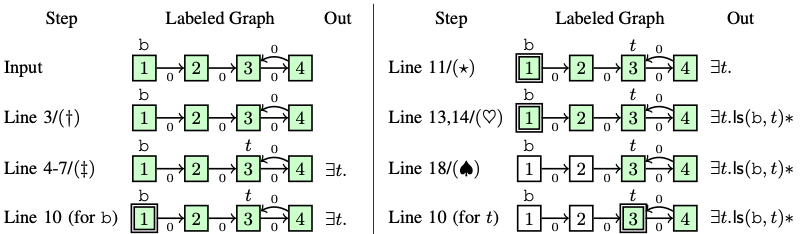
\includegraphics[width=\columnwidth]{Images/Bug1-3.png}}
\label{icml-historical}
\end{center}
\vskip -0.2in
\end{figure}

\begin{figure}[ht]
\vskip 0.2in
\begin{center}
\centerline{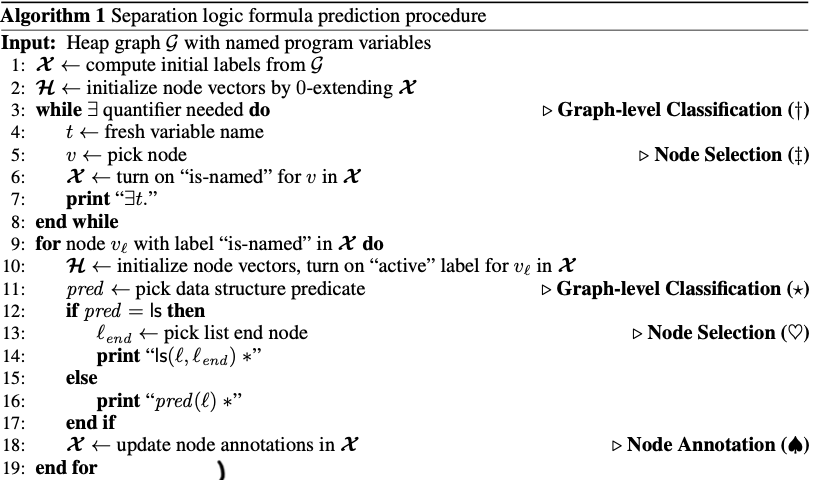
\includegraphics[width=\columnwidth]{Images/Bug1-4.png}}
\label{icml-historical}
\end{center}
\vskip -0.2in
\end{figure}

The authors use the full GGS-NN model where F$_o^{(k)}$ and F$_o^{(k)}$ have separate propagation models for 10 times steps and use D=16 dimensional node represntations. To make batch predictions, run one GGS-NN for each graph simultaneously. For each prediction step, the outputs of all the GGS-NNs at that step across the batch of graphs are aggregated. For node selection outputs, the common named variables link nodes on different graphs togeter, which is the key for aggregating predictions in a batch. Compute the score for a particular named variable t as $o_t = \sum_g o_{V_g(t)}^g$, where $V_g(t)$ maps variable name t to a node in graph g, and $o_{V_g(t)}^g$ is the output score for named variable t in graph g. When applying a softmax over all names using o$_t$ as scores, this is equivalent to a model that computes p(toselect = t) = $\prod _g p_g(toselect = V_g(t))$. For graph-level classification outputs, add up scores of a particular class across the batch of graphs, or equivalently compute p(class = k) =$\prod _g p_g$(class = k). Node annotation outputs are updated for each graph independently as different graphs have completely different set of nodes.
\subsubsection{Results.}
On comparision to GGS-NN-based model with a method developed earlier. The earlier approach treats each prediction step as standard classification, and requires complex, manual, problem-specific feature engineering, to achieve an accuracy of 89.11 percent. In contrast, this new model was trained with no feature engineering and very little domain knowledge and achieved an accuracy of 89.96 percent.
\subsection{DBN}
Specifically, this paper leverages Deep Belief Network (DBN) to automatically learn semantic features from token vectors extracted from programs’ Abstract Syntax Trees (ASTs). The code is published it https://github.com/mingkaic/defector.

The authors refer to the set of instances used for building models as the training set, whereas the set of instances used to evaluate the trained models as the test set. When performing within-project defect prediction (following existing work , they call this WPDP), the training and test sets are from the same project A. When performing cross- project defect prediction (following existing work [41] they call this CPDP), prediction models are trained by training set from a project A (source), and test set is from a different project B (target).
In this study, the authors examine the performance of learned semantic features on both WPDP and CPDP.
\subsubsection{DBN formulation}
DBN contains one input layer and several hidden layers, and the top layer is the output layer that used as features to represent input data. Each layer consists of several stochastic nodes. The number of hidden layers and the number of nodes in each layer vary depending on users’ demand. In this study, the size of learned semantic features is the number of nodes in the top layer. The idea of DBN is to enable the network to reconstruct the input data using generated features by adjusting weights between nodes in different layers.
DBN models the joint distribution between input layer and the hidden layers as follows:

\begin{math}
P(x,h^1,....h^l) = P(x,h^1)(\prod_{k=1}^l P(h^k|h^{k+1}))
\end{math}

where x is the data vector from input layer, l is the number of hidden layers, and h$^k$ is the data vector of k$^{th}$ layer (1 $\leq$ k $\leq$ l). $P(h^k|h^{k+1})$ is a conditional distribution for the adjacent k and k + 1 layer. To calculate $P(h^k|h^{k+1})$, each pair of two adjacent layers in DBN are trained as a Restricted Boltzmann Machines (RBM). A RBM is a two-layer, undirected, bipartite graphical model where the first layer consists of observed data variables, referred to as visible nodes, and the second layer consists of latent variables, referred to as hidden nodes. $P(h^k|h^{k+1})$ can be efficiently calculated as:

\begin{math}
P(h^k|h^{k+1}) = \prod_{j=1}^{n_k} P(h^k_j|h^{k+1})
\end{math}

\begin{math}
P(h^k_j|h^{k+1}) = sigm(b_j^k + \sum_{a=1}^{n_{k+1}} W^k_{aj}h^{k+1}_a
\end{math} 

where n$_k$ is the number of node in layer k, sigm(c) = $1/(1+x^{-c})$, b is a bias matrix, b$^k_j$ is the bias for node j of layer k, and W$^k$ is the weight matrix between layer k and k + 1.
DBN automatically learns W and b matrices using an iteration process. W and b are updated via log-likelihood stochastic gradient descent:

\begin{math}
W_{ij}(t+1) = W_{ij}(t) + \eta(\partial log(P(v|h)))/(\partial W_{ij})
\end{math}

\begin{math}
b_k^o(t+1) = b_k^o(t) + \eta(\partial log(P(v|h)))/(\partial b_k^o)
\end{math}

where t is the t$^{th}$ iteration, $\eta$ is the learning rate, $P(v|h)$ is the probability of the visible layer of a RBM given the hidden layer, i and j are two nodes in different layers of the RBM, Wij is the weight between the two nodes, and $b_k^o$ is the bias on the node o in layer k. To train the network, one first initializes all W matrices between two layers via RBM and sets the biases b to 0. They can be well-tuned with respect to a specific criterion. They use the number of training iterations as the criterion for tuning W and b. The well-tuned W and b are used to set up a DBN for generating semantic features for both training and test data.
\subsubsection{Approach}
Their approach first extracts a vector of tokens from the source code of each file in both the training and test sets. Since DBN requires input data in the form of integer vectors, a mapping is built between integers and tokens and convert the token vectors to integer vectors. To generate semantic features, the integer vectors of the training set are used to build a DBN. Then, the DBN is used to automatically generate semantic features from the integer vectors of the training and test sets. Finally, based on the generated semantic features, defect prediction models are built from the training set, and evaluate their performance on the test set.

AST nodes are excluded that are not one of these three categories, such as assignment and intrinsic type declaration, because they are often method-specific or class-specific, which may not be generalizable to the whole project. Adding them may dilute the importance of other nodes.for cross-project defect prediction, they extract all of AST nodes.

To detect and eliminate mislabeling data, and help DBN learn common knowledge between the semantic information of buggy and clean files, the edit distance similarity computation algorithm is adopted to define the distances between instances. The edit distances are sensitive to both the tokens and order among the tokens. Given two token sequences A and B, the edit distance d(A,B) is the minimum-weight series of edit operations that transform A to B. The smaller d(A, B) is, the more similar A and B are.

DBN takes only numerical vectors as inputs, and the lengths of the input vectors must be the same. To use DBN to generate semantic features by using DBN, a mapping is built between integers and tokens, and encode token vectors to integer vectors. Each token has a unique integer identifier while different method names and class names will be treated as different tokens. Since integer vectors may have different lengths, 0 is appended to the integer vectors to make all the lengths consistent and equal to the length of the longest vector. Adding zeros does not affect the results, and it is simply a representation transformation to make the vectors acceptable by DBN

To generate semantic features for distinguishing buggy and clean files, DBNis trained by using the training data. To train an effective DBN for learning semantic features, three parameters are tuned, which are: 1) the number of hidden layers, 2) the number of nodes in each hidden layer, and 3) the number of training iterations. Existing work that leveraged DBN to generate features for NLP and image recognition reported that the performance of DBN-generated features is sensitive to these parameters. The number of nodes to be the same in each layer. Through these hidden layers and nodes, DBN obtains characteristics that are difficult to be observed but are capable of capturing semantic differences. For each node, DBN learns probabilities of traversing from this node to the nodes of its top level. Through back- propagation validation, DBN reconstructs the input data using generated features by adjusting weights between nodes in different layers.
DBN requires the values of input data ranging from 0 to 1, while data in input vectors can have any integer values due to mapping approach. To satisfy the input range requirement, they normalize the values in the data vectors of the training and test sets by using min-max normalization.

After training a DBN, both the weights w and the biases b are fixed. The authors input the normalized integer vectors of the training data and the test data into the DBN respectively, and then obtain semantic features for the training and test data from the output layer of the DBN.
This leads to the following table and graphs for results.

\begin{figure}[ht]
\vskip 0.2in
\begin{center}
\centerline{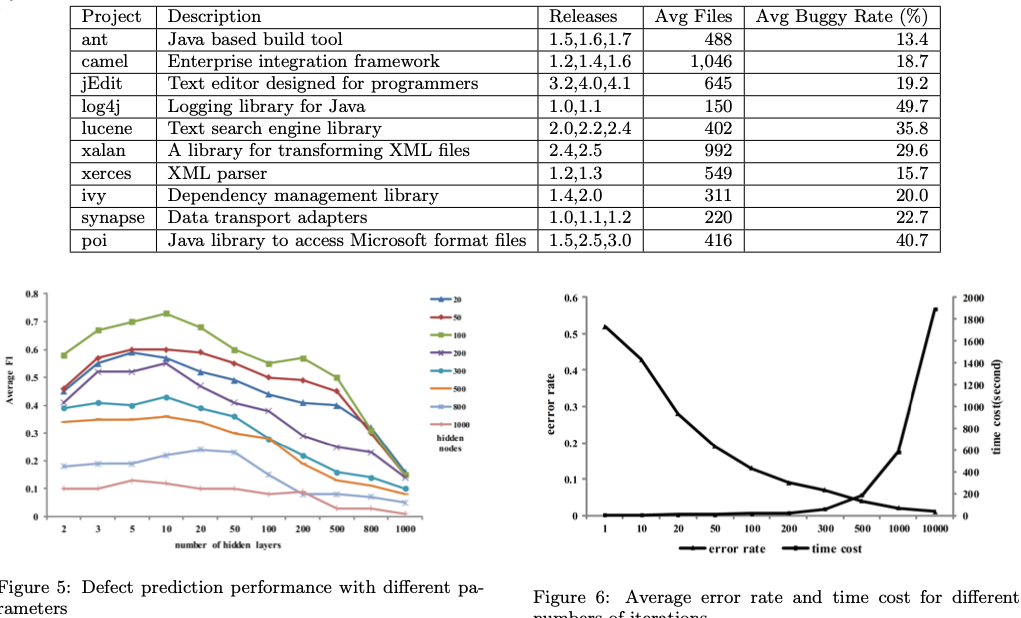
\includegraphics[width=\columnwidth]{Images/Bug2-1.png}}
\label{icml-historical}
\end{center}
\vskip -0.2in
\end{figure}

\section{Electronic Submission}
\label{submission}

Submission to ICML 2021 will be entirely electronic, via a web site
(not email). Information about the submission process and \LaTeX\ templates
are available on the conference web site at:
\begin{center}
\textbf{\texttt{http://icml.cc/}}
\end{center}

The guidelines below will be enforced for initial submissions and
camera-ready copies. Here is a brief summary:
\begin{itemize}
\item Submissions must be in PDF\@.
\item Submitted papers can be up to eight pages long, not including references, plus unlimited space for references. Accepted papers can be up to nine pages long, not including references, to allow authors to address reviewer comments. Any paper exceeding this length will automatically be rejected. 
\item \textbf{Do not include author information or acknowledgements} in your
    initial submission.
\item Your paper should be in \textbf{10 point Times font}.
\item Make sure your PDF file only uses Type-1 fonts.
\item Place figure captions \emph{under} the figure (and omit titles from inside
    the graphic file itself). Place table captions \emph{over} the table.
\item References must include page numbers whenever possible and be as complete
    as possible. Place multiple citations in chronological order.
\item Do not alter the style template; in particular, do not compress the paper
    format by reducing the vertical spaces.
\item Keep your abstract brief and self-contained, one paragraph and roughly
    4--6 sentences. Gross violations will require correction at the
    camera-ready phase. The title should have content words capitalized.
\end{itemize}

\subsection{Submitting Papers}

\textbf{Paper Deadline:} The deadline for paper submission that is
advertised on the conference website is strict. If your full,
anonymized, submission does not reach us on time, it will not be
considered for publication. 

\textbf{Anonymous Submission:} ICML uses double-blind review: no identifying
author information may appear on the title page or in the paper
itself. Section~\ref{author info} gives further details.

\textbf{Simultaneous Submission:} ICML will not accept any paper which,
at the time of submission, is under review for another conference or
has already been published. This policy also applies to papers that
overlap substantially in technical content with conference papers
under review or previously published. ICML submissions must not be
submitted to other conferences and journals during ICML's review
period.
%Authors may submit to ICML substantially different versions of journal papers
%that are currently under review by the journal, but not yet accepted
%at the time of submission.
Informal publications, such as technical
reports or papers in workshop proceedings which do not appear in
print, do not fall under these restrictions.

\medskip

Authors must provide their manuscripts in \textbf{PDF} format.
Furthermore, please make sure that files contain only embedded Type-1 fonts
(e.g.,~using the program \texttt{pdffonts} in linux or using
File/DocumentProperties/Fonts in Acrobat). Other fonts (like Type-3)
might come from graphics files imported into the document.

Authors using \textbf{Word} must convert their document to PDF\@. Most
of the latest versions of Word have the facility to do this
automatically. Submissions will not be accepted in Word format or any
format other than PDF\@. Really. We're not joking. Don't send Word.

Those who use \textbf{\LaTeX} should avoid including Type-3 fonts.
Those using \texttt{latex} and \texttt{dvips} may need the following
two commands:

{\footnotesize
\begin{verbatim}
dvips -Ppdf -tletter -G0 -o paper.ps paper.dvi
ps2pdf paper.ps
\end{verbatim}}
It is a zero following the ``-G'', which tells dvips to use
the config.pdf file. Newer \TeX\ distributions don't always need this
option.

Using \texttt{pdflatex} rather than \texttt{latex}, often gives better
results. This program avoids the Type-3 font problem, and supports more
advanced features in the \texttt{microtype} package.

\textbf{Graphics files} should be a reasonable size, and included from
an appropriate format. Use vector formats (.eps/.pdf) for plots,
lossless bitmap formats (.png) for raster graphics with sharp lines, and
jpeg for photo-like images.

The style file uses the \texttt{hyperref} package to make clickable
links in documents. If this causes problems for you, add
\texttt{nohyperref} as one of the options to the \texttt{icml2021}
usepackage statement.


\subsection{Submitting Final Camera-Ready Copy}

The final versions of papers accepted for publication should follow the
same format and naming convention as initial submissions, except that
author information (names and affiliations) should be given. See
Section~\ref{final author} for formatting instructions.

The footnote, ``Preliminary work. Under review by the International
Conference on Machine Learning (ICML). Do not distribute.'' must be
modified to ``\textit{Proceedings of the
$\mathit{38}^{th}$ International Conference on Machine Learning},
Online, PMLR 139, 2021.
Copyright 2021 by the author(s).''

For those using the \textbf{\LaTeX} style file, this change (and others) is
handled automatically by simply changing
$\mathtt{\backslash usepackage\{icml2021\}}$ to
$$\mathtt{\backslash usepackage[accepted]\{icml2021\}}$$
Authors using \textbf{Word} must edit the
footnote on the first page of the document themselves.

Camera-ready copies should have the title of the paper as running head
on each page except the first one. The running title consists of a
single line centered above a horizontal rule which is $1$~point thick.
The running head should be centered, bold and in $9$~point type. The
rule should be $10$~points above the main text. For those using the
\textbf{\LaTeX} style file, the original title is automatically set as running
head using the \texttt{fancyhdr} package which is included in the ICML
2021 style file package. In case that the original title exceeds the
size restrictions, a shorter form can be supplied by using

\verb|\icmltitlerunning{...}|

just before $\mathtt{\backslash begin\{document\}}$.
Authors using \textbf{Word} must edit the header of the document themselves.

\section{Format of the Paper}

All submissions must follow the specified format.

\subsection{Dimensions}




The text of the paper should be formatted in two columns, with an
overall width of 6.75~inches, height of 9.0~inches, and 0.25~inches
between the columns. The left margin should be 0.75~inches and the top
margin 1.0~inch (2.54~cm). The right and bottom margins will depend on
whether you print on US letter or A4 paper, but all final versions
must be produced for US letter size.

The paper body should be set in 10~point type with a vertical spacing
of 11~points. Please use Times typeface throughout the text.

\subsection{Title}

The paper title should be set in 14~point bold type and centered
between two horizontal rules that are 1~point thick, with 1.0~inch
between the top rule and the top edge of the page. Capitalize the
first letter of content words and put the rest of the title in lower
case.

\subsection{Author Information for Submission}
\label{author info}

ICML uses double-blind review, so author information must not appear. If
you are using \LaTeX\/ and the \texttt{icml2021.sty} file, use
\verb+\icmlauthor{...}+ to specify authors and \verb+\icmlaffiliation{...}+ to specify affiliations. (Read the TeX code used to produce this document for an example usage.) The author information
will not be printed unless \texttt{accepted} is passed as an argument to the
style file.
Submissions that include the author information will not
be reviewed.

\subsubsection{Self-Citations}

If you are citing published papers for which you are an author, refer
to yourself in the third person. In particular, do not use phrases
that reveal your identity (e.g., ``in previous work \cite{langley00}, we
have shown \ldots'').

Do not anonymize citations in the reference section. The only exception are manuscripts that are
not yet published (e.g., under submission). If you choose to refer to
such unpublished manuscripts \cite{anonymous}, anonymized copies have
to be submitted
as Supplementary Material via CMT\@. However, keep in mind that an ICML
paper should be self contained and should contain sufficient detail
for the reviewers to evaluate the work. In particular, reviewers are
not required to look at the Supplementary Material when writing their
review.

\subsubsection{Camera-Ready Author Information}
\label{final author}

If a paper is accepted, a final camera-ready copy must be prepared.
%
For camera-ready papers, author information should start 0.3~inches below the
bottom rule surrounding the title. The authors' names should appear in 10~point
bold type, in a row, separated by white space, and centered. Author names should
not be broken across lines. Unbolded superscripted numbers, starting 1, should
be used to refer to affiliations.

Affiliations should be numbered in the order of appearance. A single footnote
block of text should be used to list all the affiliations. (Academic
affiliations should list Department, University, City, State/Region, Country.
Similarly for industrial affiliations.)

Each distinct affiliations should be listed once. If an author has multiple
affiliations, multiple superscripts should be placed after the name, separated
by thin spaces. If the authors would like to highlight equal contribution by
multiple first authors, those authors should have an asterisk placed after their
name in superscript, and the term ``\textsuperscript{*}Equal contribution"
should be placed in the footnote block ahead of the list of affiliations. A
list of corresponding authors and their emails (in the format Full Name
\textless{}email@domain.com\textgreater{}) can follow the list of affiliations.
Ideally only one or two names should be listed.

A sample file with author names is included in the ICML2021 style file
package. Turn on the \texttt{[accepted]} option to the stylefile to
see the names rendered. All of the guidelines above are implemented
by the \LaTeX\ style file.

\subsection{Abstract}

The paper abstract should begin in the left column, 0.4~inches below the final
address. The heading `Abstract' should be centered, bold, and in 11~point type.
The abstract body should use 10~point type, with a vertical spacing of
11~points, and should be indented 0.25~inches more than normal on left-hand and
right-hand margins. Insert 0.4~inches of blank space after the body. Keep your
abstract brief and self-contained, limiting it to one paragraph and roughly 4--6
sentences. Gross violations will require correction at the camera-ready phase.

\subsection{Partitioning the Text}

You should organize your paper into sections and paragraphs to help
readers place a structure on the material and understand its
contributions.

\subsubsection{Sections and Subsections}

Section headings should be numbered, flush left, and set in 11~pt bold
type with the content words capitalized. Leave 0.25~inches of space
before the heading and 0.15~inches after the heading.

Similarly, subsection headings should be numbered, flush left, and set
in 10~pt bold type with the content words capitalized. Leave
0.2~inches of space before the heading and 0.13~inches afterward.

Finally, subsubsection headings should be numbered, flush left, and
set in 10~pt small caps with the content words capitalized. Leave
0.18~inches of space before the heading and 0.1~inches after the
heading.

Please use no more than three levels of headings.

\subsubsection{Paragraphs and Footnotes}

Within each section or subsection, you should further partition the
paper into paragraphs. Do not indent the first line of a given
paragraph, but insert a blank line between succeeding ones.

You can use footnotes\footnote{Footnotes
should be complete sentences.} to provide readers with additional
information about a topic without interrupting the flow of the paper.
Indicate footnotes with a number in the text where the point is most
relevant. Place the footnote in 9~point type at the bottom of the
column in which it appears. Precede the first footnote in a column
with a horizontal rule of 0.8~inches.\footnote{Multiple footnotes can
appear in each column, in the same order as they appear in the text,
but spread them across columns and pages if possible.}

\begin{figure}[ht]
\vskip 0.2in
\begin{center}
\centerline{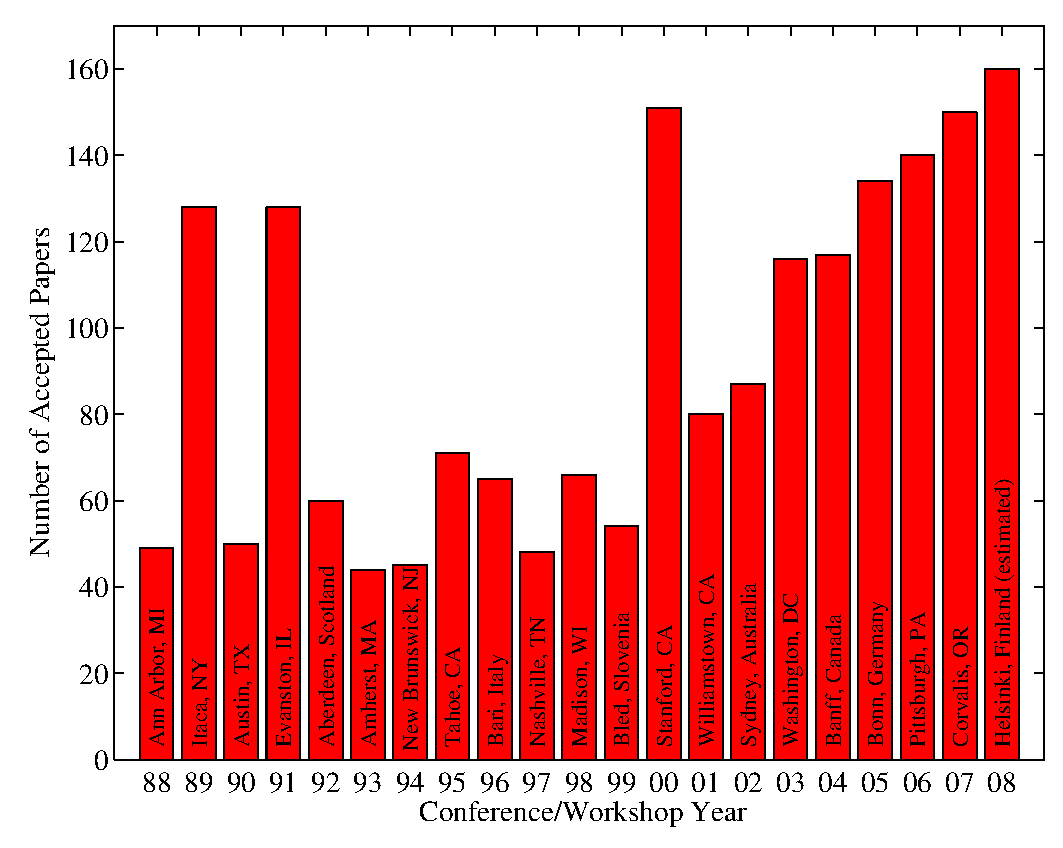
\includegraphics[width=\columnwidth]{icml_numpapers}}
\caption{Historical locations and number of accepted papers for International
Machine Learning Conferences (ICML 1993 -- ICML 2008) and International
Workshops on Machine Learning (ML 1988 -- ML 1992). At the time this figure was
produced, the number of accepted papers for ICML 2008 was unknown and instead
estimated.}
\label{icml-historical}
\end{center}
\vskip -0.2in
\end{figure}

\subsection{Figures}

You may want to include figures in the paper to illustrate
your approach and results. Such artwork should be centered,
legible, and separated from the text. Lines should be dark and at
least 0.5~points thick for purposes of reproduction, and text should
not appear on a gray background.

Label all distinct components of each figure. If the figure takes the
form of a graph, then give a name for each axis and include a legend
that briefly describes each curve. Do not include a title inside the
figure; instead, the caption should serve this function.

Number figures sequentially, placing the figure number and caption
\emph{after} the graphics, with at least 0.1~inches of space before
the caption and 0.1~inches after it, as in
Figure~\ref{icml-historical}. The figure caption should be set in
9~point type and centered unless it runs two or more lines, in which
case it should be flush left. You may float figures to the top or
bottom of a column, and you may set wide figures across both columns
(use the environment \texttt{figure*} in \LaTeX). Always place
two-column figures at the top or bottom of the page.

\subsection{Algorithms}

If you are using \LaTeX, please use the ``algorithm'' and ``algorithmic''
environments to format pseudocode. These require
the corresponding stylefiles, algorithm.sty and
algorithmic.sty, which are supplied with this package.
Algorithm~\ref{alg:example} shows an example.

\begin{algorithm}[tb]
   \caption{Bubble Sort}
   \label{alg:example}
\begin{algorithmic}
   \STATE {\bfseries Input:} data $x_i$, size $m$
   \REPEAT
   \STATE Initialize $noChange = true$.
   \FOR{$i=1$ {\bfseries to} $m-1$}
   \IF{$x_i > x_{i+1}$}
   \STATE Swap $x_i$ and $x_{i+1}$
   \STATE $noChange = false$
   \ENDIF
   \ENDFOR
   \UNTIL{$noChange$ is $true$}
\end{algorithmic}
\end{algorithm}

\subsection{Tables}

You may also want to include tables that summarize material. Like
figures, these should be centered, legible, and numbered consecutively.
However, place the title \emph{above} the table with at least
0.1~inches of space before the title and the same after it, as in
Table~\ref{sample-table}. The table title should be set in 9~point
type and centered unless it runs two or more lines, in which case it
should be flush left.

% Note use of \abovespace and \belowspace to get reasonable spacing
% above and below tabular lines.

\begin{table}[t]
\caption{Classification accuracies for naive Bayes and flexible
Bayes on various data sets.}
\label{sample-table}
\vskip 0.15in
\begin{center}
\begin{small}
\begin{sc}
\begin{tabular}{lcccr}
\toprule
Data set & Naive & Flexible & Better? \\
\midrule
Breast    & 95.9$\pm$ 0.2& 96.7$\pm$ 0.2& $\surd$ \\
Cleveland & 83.3$\pm$ 0.6& 80.0$\pm$ 0.6& $\times$\\
Glass2    & 61.9$\pm$ 1.4& 83.8$\pm$ 0.7& $\surd$ \\
Credit    & 74.8$\pm$ 0.5& 78.3$\pm$ 0.6&         \\
Horse     & 73.3$\pm$ 0.9& 69.7$\pm$ 1.0& $\times$\\
Meta      & 67.1$\pm$ 0.6& 76.5$\pm$ 0.5& $\surd$ \\
Pima      & 75.1$\pm$ 0.6& 73.9$\pm$ 0.5&         \\
Vehicle   & 44.9$\pm$ 0.6& 61.5$\pm$ 0.4& $\surd$ \\
\bottomrule
\end{tabular}
\end{sc}
\end{small}
\end{center}
\vskip -0.1in
\end{table}

Tables contain textual material, whereas figures contain graphical material.
Specify the contents of each row and column in the table's topmost
row. Again, you may float tables to a column's top or bottom, and set
wide tables across both columns. Place two-column tables at the
top or bottom of the page.

\subsection{Citations and References}

Please use APA reference format regardless of your formatter
or word processor. If you rely on the \LaTeX\/ bibliographic
facility, use \texttt{natbib.sty} and \texttt{icml2021.bst}
included in the style-file package to obtain this format.

Citations within the text should include the authors' last names and
year. If the authors' names are included in the sentence, place only
the year in parentheses, for example when referencing Arthur Samuel's
pioneering work \yrcite{Samuel59}. Otherwise place the entire
reference in parentheses with the authors and year separated by a
comma \cite{Samuel59}. List multiple references separated by
semicolons \cite{kearns89,Samuel59,mitchell80}. Use the `et~al.'
construct only for citations with three or more authors or after
listing all authors to a publication in an earlier reference \cite{MachineLearningI}.

Authors should cite their own work in the third person
in the initial version of their paper submitted for blind review.
Please refer to Section~\ref{author info} for detailed instructions on how to
cite your own papers.

Use an unnumbered first-level section heading for the references, and use a
hanging indent style, with the first line of the reference flush against the
left margin and subsequent lines indented by 10 points. The references at the
end of this document give examples for journal articles \cite{Samuel59},
conference publications \cite{langley00}, book chapters \cite{Newell81}, books
\cite{DudaHart2nd}, edited volumes \cite{MachineLearningI}, technical reports
\cite{mitchell80}, and dissertations \cite{kearns89}.

Alphabetize references by the surnames of the first authors, with
single author entries preceding multiple author entries. Order
references for the same authors by year of publication, with the
earliest first. Make sure that each reference includes all relevant
information (e.g., page numbers).

Please put some effort into making references complete, presentable, and
consistent. If using bibtex, please protect capital letters of names and
abbreviations in titles, for example, use \{B\}ayesian or \{L\}ipschitz
in your .bib file.

\section*{Software and Data}

If a paper is accepted, we strongly encourage the publication of software and data with the
camera-ready version of the paper whenever appropriate. This can be
done by including a URL in the camera-ready copy. However, \textbf{do not}
include URLs that reveal your institution or identity in your
submission for review. Instead, provide an anonymous URL or upload
the material as ``Supplementary Material'' into the CMT reviewing
system. Note that reviewers are not required to look at this material
when writing their review.

% Acknowledgements should only appear in the accepted version.
\section*{Acknowledgements}

\textbf{Do not} include acknowledgements in the initial version of
the paper submitted for blind review.

If a paper is accepted, the final camera-ready version can (and
probably should) include acknowledgements. In this case, please
place such acknowledgements in an unnumbered section at the
end of the paper. Typically, this will include thanks to reviewers
who gave useful comments, to colleagues who contributed to the ideas,
and to funding agencies and corporate sponsors that provided financial
support.


% In the unusual situation where you want a paper to appear in the
% references without citing it in the main text, use \nocite
\nocite{langley00}

\bibliography{main}
\bibliographystyle{icml2021}


%%%%%%%%%%%%%%%%%%%%%%%%%%%%%%%%%%%%%%%%%%%%%%%%%%%%%%%%%%%%%%%%%%%%%%%%%%%%%%%
%%%%%%%%%%%%%%%%%%%%%%%%%%%%%%%%%%%%%%%%%%%%%%%%%%%%%%%%%%%%%%%%%%%%%%%%%%%%%%%
% DELETE THIS PART. DO NOT PLACE CONTENT AFTER THE REFERENCES!
%%%%%%%%%%%%%%%%%%%%%%%%%%%%%%%%%%%%%%%%%%%%%%%%%%%%%%%%%%%%%%%%%%%%%%%%%%%%%%%
%%%%%%%%%%%%%%%%%%%%%%%%%%%%%%%%%%%%%%%%%%%%%%%%%%%%%%%%%%%%%%%%%%%%%%%%%%%%%%%
\appendix
\section{Do \emph{not} have an appendix here}

\textbf{\emph{Do not put content after the references.}}
%
Put anything that you might normally include after the references in a separate
supplementary file.

We recommend that you build supplementary material in a separate document.
If you must create one PDF and cut it up, please be careful to use a tool that
doesn't alter the margins, and that doesn't aggressively rewrite the PDF file.
pdftk usually works fine. 

\textbf{Please do not use Apple's preview to cut off supplementary material.} In
previous years it has altered margins, and created headaches at the camera-ready
stage. 
%%%%%%%%%%%%%%%%%%%%%%%%%%%%%%%%%%%%%%%%%%%%%%%%%%%%%%%%%%%%%%%%%%%%%%%%%%%%%%%
%%%%%%%%%%%%%%%%%%%%%%%%%%%%%%%%%%%%%%%%%%%%%%%%%%%%%%%%%%%%%%%%%%%%%%%%%%%%%%%


\end{document}


% This document was modified from the file originally made available by
% Pat Langley and Andrea Danyluk for ICML-2K. This version was created
% by Iain Murray in 2018, and modified by Alexandre Bouchard in
% 2019 and 2021. Previous contributors include Dan Roy, Lise Getoor and Tobias
% Scheffer, which was slightly modified from the 2010 version by
% Thorsten Joachims & Johannes Fuernkranz, slightly modified from the
% 2009 version by Kiri Wagstaff and Sam Roweis's 2008 version, which is
% slightly modified from Prasad Tadepalli's 2007 version which is a
% lightly changed version of the previous year's version by Andrew
% Moore, which was in turn edited from those of Kristian Kersting and
% Codrina Lauth. Alex Smola contributed to the algorithmic style files.
